% This is the Duke University Statistical Science LaTeX thesis template.
% It has been adapted from the Reed College LaTeX thesis template. The
% adaptation was done by Mine Cetinkaya-Rundel (MCR). Some of the comments
% that are specific to Reed College have been removed.
%
% Most of the work on the original Reed College document class and template
% was done by Sam Noble (SN). Later comments etc. by Ben Salzberg (BTS).
% Additional restructuring and APA support by Jess Youngberg (JY).
%
% See https://www.reed.edu/cis/help/latex/ for help. There are a
% great bunch of help pages there, with notes on
% getting started, bibtex, etc. Go there and read it if you're not
% already familiar with LaTeX.
%
% Any line that starts with a percent symbol is a comment.
% They won't show up in the document, and are useful for notes
% to yourself and explaining commands.
% Commenting also removes a line from the document;
% very handy for troubleshooting problems. -BTS

%%
%% Preamble
%%
% \documentclass{<something>} must begin each LaTeX document
\documentclass[12pt,twoside]{dukestatscithesis}
% Packages are extensions to the basic LaTeX functions. Whatever you
% want to typeset, there is probably a package out there for it.
% Chemistry (chemtex), screenplays, you name it.
% Check out CTAN to see: http://www.ctan.org/
%%
\usepackage{graphicx,latexsym}
\usepackage{amsmath}
\usepackage{amssymb,amsthm}
\usepackage{longtable,booktabs,setspace}
\usepackage{chemarr} %% Useful for one reaction arrow, useless if you're not a chem major
\usepackage[hyphens]{url}
% Added by CII
\usepackage{hyperref}
\usepackage{lmodern}
\usepackage{float}
\floatplacement{figure}{H}
% End of CII addition
\usepackage{rotating}

% Next line commented out by CII
%%% \usepackage{natbib}
% Comment out the natbib line above and uncomment the following two lines to use the new
% biblatex-chicago style, for Chicago A. Also make some changes at the end where the
% bibliography is included.
%\usepackage{biblatex-chicago}
%\bibliography{thesis}


% Added by CII (Thanks, Hadley!)
% Use ref for internal links
\renewcommand{\hyperref}[2][???]{\autoref{#1}}
\def\chapterautorefname{Chapter}
\def\sectionautorefname{Section}
\def\subsectionautorefname{Subsection}
% End of CII addition

% Added by CII
\usepackage{caption}
\captionsetup{width=5in}
% End of CII addition

% \usepackage{times} % other fonts are available like times, bookman, charter, palatino


% To pass between YAML and LaTeX the dollar signs are added by CII
\title{Bayesian Analysis of Player Performance over Time}
\author{Nathaniel Brown}
% The month and year that you submit your FINAL draft TO THE LIBRARY (May or December)
\date{May 2018}
\advisor{Mike West}
\institution{Duke University}
\degree{Bachelor of Science in Statistical Science}
\committeememberone{Merlise Clyde}
\committeemembertwo{Cliburn Chan}
\dus{Mine Cetinkaya-Rundel}
%If you have two advisors for some reason, you can use the following
% Uncommented out by CII
% End of CII addition

%%% Remember to use the correct department!
\department{Department of Statistical Science}

% Added by CII
%%% Copied from knitr
%% maxwidth is the original width if it's less than linewidth
%% otherwise use linewidth (to make sure the graphics do not exceed the margin)
\makeatletter
\def\maxwidth{ %
  \ifdim\Gin@nat@width>\linewidth
    \linewidth
  \else
    \Gin@nat@width
  \fi
}
\makeatother

\renewcommand{\contentsname}{Table of Contents}
% End of CII addition

\setlength{\parskip}{0pt}

% Added by CII
  %\setlength{\parskip}{\baselineskip}
  \usepackage[parfill]{parskip}

\providecommand{\tightlist}{%
  \setlength{\itemsep}{0pt}\setlength{\parskip}{0pt}}

\Acknowledgements{
A special thank you to Kevin Cullen, Basketball Director of Information
Technology for the Duke Men's Basketball team, for providing data for
this research.
}

\Dedication{
Insert a real dedication. (optional)
}

\Preface{

}

\Abstract{
\chapter{Abstract}\label{abstract}

This study is an investigation of Bayesian statistical models and
analyses for problems arising in shooting a basketball. The dataset is
from the Duke Men's Basketball team's player-tracking data, which is
recorded on the SportVU cameras from STATS, LLC. Goals are to explore,
develop, and apply Bayesian models to existing and new data on shooting
outcomes. In addition, we want to understand and evaluate questions of
inherent random variation, changes over time in shooting performance,
and issues related to the ``Hot Hand'' concept in sports.

The models we use to investigate this data are a Bayesian logistic
generalized linear model, a hierarchical model with mixed effects on the
shooter identity, and a discounted likelihood model that reduces the
influence of shots as their time difference from the current shot
increases.

Our results so far show that the best-fitting model is \ldots{}
}

% End of CII addition
%%
%% End Preamble
%%
%

\usepackage{amsthm}
\newtheorem{theorem}{Theorem}[chapter]
\newtheorem{lemma}{Lemma}[chapter]
\theoremstyle{definition}
\newtheorem{definition}{Definition}[chapter]
\newtheorem{corollary}{Corollary}[chapter]
\newtheorem{proposition}{Proposition}[chapter]
\theoremstyle{definition}
\newtheorem{example}{Example}[chapter]
\theoremstyle{definition}
\newtheorem{exercise}{Exercise}[chapter]
\theoremstyle{remark}
\newtheorem*{remark}{Remark}
\newtheorem*{solution}{Solution}
\begin{document}

% Everything below added by CII
  \maketitle

\frontmatter % this stuff will be roman-numbered
\pagestyle{empty} % this removes page numbers from the frontmatter
  \begin{acknowledgements}
    A special thank you to Kevin Cullen, Basketball Director of Information
    Technology for the Duke Men's Basketball team, for providing data for
    this research.
  \end{acknowledgements}

  \hypersetup{linkcolor=black}
  \setcounter{tocdepth}{2}
  \tableofcontents

  \listoftables

  \listoffigures
  \begin{abstract}
    \chapter{Abstract}\label{abstract}
    
    This study is an investigation of Bayesian statistical models and
    analyses for problems arising in shooting a basketball. The dataset is
    from the Duke Men's Basketball team's player-tracking data, which is
    recorded on the SportVU cameras from STATS, LLC. Goals are to explore,
    develop, and apply Bayesian models to existing and new data on shooting
    outcomes. In addition, we want to understand and evaluate questions of
    inherent random variation, changes over time in shooting performance,
    and issues related to the ``Hot Hand'' concept in sports.
    
    The models we use to investigate this data are a Bayesian logistic
    generalized linear model, a hierarchical model with mixed effects on the
    shooter identity, and a discounted likelihood model that reduces the
    influence of shots as their time difference from the current shot
    increases.
    
    Our results so far show that the best-fitting model is \ldots{}
  \end{abstract}
  \begin{dedication}
    Insert a real dedication. (optional)
  \end{dedication}
\mainmatter % here the regular arabic numbering starts
\pagestyle{fancyplain} % turns page numbering back on

\chapter*{Introduction}\label{introduction}
\addcontentsline{toc}{chapter}{Introduction}

In the sport of basketball, points are awarded by the binary event of
shooting the ball into the goal. Some factors we consider that may
affect the success rate include the location of the shooter, the
individual skill of the shooter, whether the shooter is playing on his
home court or on an away court, and the shooting success in recent
surrounding games. There have been previous studies investigating the
effect of recent shooting success on current shooting success, and the
results vary. For example, Gilovich, Vallone, \& Tversky (1985) use
Walf-Wolfowitz run tests, autocorrelation tests on consecutive shot
attempts, goodness-of-fit tests for the distribution of successes, and
paired t-tests comparing the mean of makes following a make to that of
makes following a miss. These statistical tests did not detect
significant evidence supporting streakiness in basketball shooting data.
In addition, Ryan Wetzels (2016) found evidence that a Hidden Markov
Model with two states (representing a high shot success rate and a low
rate) better fits Shaquille O'Neal's free throw shooting data than a
Binomial model with one constant state. Bar-Eli, Avugos, \& Raab (2006)
completed a review of previous statistical papers whose authors research
the concept of streaky success rates in data with a binomial response;
the applications include basketball shooting, baseball hitting, baseball
pitching, horeshoe, cognitive science, and economics. They summarize 11
papers that support evidence of streakiness in binomial data, and 13
that do not.

The purpose of this paper is to investigate Bayesian modelling
techniques shooting data, and to learn more about time-dependency in
shooting data.

\chapter{Abstract}\label{abstract}

This study is an investigation of Bayesian statistical models and
analyses for problems arising in shooting a basketball. The dataset is
from the Duke Men's Basketball team's player-tracking data, which is
recorded on the SportVU cameras from STATS, LLC. Goals are to explore,
develop, and apply Bayesian models to existing and new data on shooting
outcomes. In addition, we want to understand and evaluate questions of
inherent random variation, changes over time in shooting performance,
and issues related to the ``Hot Hand'' concept in sports.

The models we use to investigate this data are a Bayesian logistic
generalized linear model, a hierarchical model with mixed effects on the
shooter identity, and a discounted likelihood model that reduces the
influence of shots as their time difference from the current shot
increases.

Our results so far show that the best-fitting model is \ldots{}

\chapter{Literature Review}\label{litreview}

\section{how do I get the full citations to show up and not just last
name and
year?}\label{how-do-i-get-the-full-citations-to-show-up-and-not-just-last-name-and-year}

Albert (1993)

In this paper, Albert uses a Markov switching model to analyze
streakiness in baseball pitching data. He concludes that a few players
exhibit streakiness, but not enough to reject the null hypothesis. An
exploratory technique that we take from this paper is to examine the
peaks and valleys in a moving average plot to observe streakiness. A
strength of this paper is that Albert controls for situational variables
such as home field advantage, the handedness of the pitcher, and the
runners on the bases.

Albert (2013)

In this paper, Albert analyzes streakiness in baseball hitting data. His
analysis techniques include using Bayes Factors to compare models of the
form \(f(y_j|p_j) = p_j(1-p_j)^{y_j}, y_j = 0,1,2,...\); a consistent
model with a constant \(p_j\), and a streaky model with a varying
\(p_j\) from a beta distribution. A useful insight that we apply to this
paper is the concept that the existence of streakiness depends on the
definition of ``success'' in binary outcome data. He found substantially
more evidence for streakiness for when a success was coded as ``not a
strikeout'' instead of a ``hit''. From this paper, we learn that the
organization of the data can affect the outcomes, and a technique for
comparing Bayesian models.

Albert \& Williamson (1999)

In this paper, Jim Albert attempts to improve upon the low-powered tests
of Gilovich, Vallone, and Tverky's 1985 paper on the Hot Hand. Albert
formally defines ``streakiness'' as the presence of nonstationarity
(nonconstant probability between trials) or autocorrelation (sequential
dependency). Albert uses Gibbs sampling to approximate posterior
densities and to simulate data, then fits two types of models on binary
data from baseball and basketball to try to characterize streakiness. He
fits an overdispersion model to detect nonstationarity, and a markov
switching model to detect sequential dependencies. While he did not
uncover strong evidence for the hot hand, one of his takeaways was that
overdispersion decreases as time goes on in basketball free throw
shooting data. A weakness of this paper is that Albert does not show the
results of both the Markov model and the overdispersion model on the
same data. We use Albert's formal definitions of streakiness as well as
his motivation for Bayesian models over frequentist tests.

Ameen \& Harrison (1984)

This journal article contains information about discounted likelihood
regression using exponential weights, which generalizes to discount
weighted estimation (DWE). There is also a section that elaborates on
how these models apply to time series. Although the material in this
book focues on data with a Normal response instead of a Binomial, we use
the concepts in this article to help explain our discounted likelihood
models in Section \textbf{number.number.number}.

Bar-Eli et al. (2006)

This paper is a review of previous hot hand research. It reviews several
papers investigating the concept of the ``hot hand'' in several sports
such as basketball, baseball, volleyball, and horseshoe, and other
fields such as cognitive science and economics. Bar-Eli, Avugos, and
Raab evaluate the datasets, the tests and statistics used, and the
conclusions of each study. Overall, the authors summarize 13 papers that
oppose the hot hand phenomenon, and 11 that support it; they also
acknowledge that the scientific evidence for the hot hand is weaker than
the evidence against it, and it is typically more controversial. Instead
of just looking to answer whether the hot hand exists, Bar-Eli, Avugos,
and Raab also examine how people define a ``hot hand'', and the
psychological factors behind the belief in it, such as the gambling and
game strategy. The strengths of this paper are that it evaluates the
strengths and weaknesses of many competing claims, and concisely
summarizes the information into a table. A weakness is that they do not
make any claim of their own. This paper is useful in this thesis because
it describes several data analysis techniques to detect streaks in a
binary sequence.

Gilovich et al. (1985)

In this research paper from \emph{Cognitive Psychology}, Thomas
Gilovich, Robert Vallone, and Amos Tversky investigate peoples' belief
in the Hot Hand in Basketball. The Hot Hand is the concept that the
probability of a success increases for trials that follow a success in a
binary sequence; in basketball, these binary events are shot attempts.
The methods in this paper include an analysis of shot attempts from the
Philadelphia 76ers of the National Basketball Association (NBA) in the
1981 season, analysis of free-throw attempts from the Boston Celtics in
the 1981 and 1982 seasons, and a controlled shooting drill using male
and female varsity basketball players at Cornell University. Statistical
techniques they used to attempt to detect streakiness in the data
included Walf-Wolfowitz run tests, autocorrelation tests on consecutive
shot attempts, goodness-of-fit tests for the distribution of successes,
and paired t-tests comparing the mean of makes following a make to that
of makes following a miss. In addition to this analysis of shooting,
this research also contained a survey of basketball fans, that gauged
how much people believed success probabilities changed given a success
or a failure. The statistical tests did not detect significant evidence
supporting the Hot Hand in basketball. The lack of statistical power in
Gilovich, Vallone, and Tversky's frequentist tests motivates the use of
Bayesian models in this thesis. Strengths of this paper include the fact
that it was one of the first research papers to analyze streakiness in
basketball data, and many future papers build off of it. Some weaknesses
in this paper are the assumptions it makes in its analysis, such as all
shots being independent of each other, and not accounting for shot
location.

Prado \& West (2010)

This textbook provides theory, applications, and examples of time series
models such Dynamic Generalized Linear Models (DGLMs). More
specifically, section 14.4 provides an example of a DGLM for a binomial
response variable. The concept of a time-varying parameter in a binomial
model is applied in this paper, through our use of discounted likelihood
models.

Ryan Wetzels (2016)

In this research paper, Wetzels conducts a simulation study to
investigate the Hot Hand Phenomenon. His analysis consists of
calculating Bayes Factors to compare evidence between a Hidden Markov
Model with two states and a binomial model with one state. He applies
this method to data from basketball foul shots and from visual
discernment tests. In the basketball data, he found that Shaquille
O'Neal's free-throws show evidence for a two-state Markov model, while
Kobe Bryant's show more evidence for a one-state binomial model. In the
data from the visual discernment tests, he found no strong evidence
supporting one model over the other. A strength of this paper is
Wetzel's formal comparison of a Bayesian Markov model to a binomial
model. A weakness is that the Bayes Factors only compare evidence
between the two models; it does not mean that either model is ``good''.
We use this paper for the specification of the Hidden Markov Model.

\chapter{Data}\label{data}

\section{Description of Dataset}\label{description-of-dataset}

The data for this analysis comes from SportVU, a player-tracking system
from STATS, LLC. that provides precise coordinates for all ten players
and the ball at a rate of 25 times per second. The Duke University Men's
Basketball team permitted us to use their SportVU data from the 2014 to
2017 basketball seasons for this project. Since the ability to record
this data depends on specialized tracking cameras, Duke does not have
this data for every game they play---only home games, and a few road
games in arenas that had the technology installed. Therefore, there is a
substantial amount of missing data between games. More specifically,
between the 2014 and 2017 seasons, the Duke Men's Basketball team played
147 games; this dataset contains 94 games, with 82 at Duke and 12 other
courts.

For our analysis, we use the following files for each game:
\begin{itemize}
\tightlist
\item
  Final Sequence Play-by-Play Optical:
\end{itemize}
This dataset comes in an a semi-structured Extensible Markup Language
(XML) file, where there is a unique element for each ``event'' (an event
is a basketball action such as a dribble, pass, shot, foul, etc.). Each
event element has attributes describing the type of event, the time of
the event, and the player who completed the action. We use these files
to uncover when a shot is attempted in a game, who attempted the shot,
and the result of the shot attempt.
\begin{itemize}
\item
  Final Sequence Optical:

  These XML files contain the locations of all ten players and the ball
  during precise time intervals within the game. Each time unit has a
  unique element, and these elements have attributes describing the
  locations. We merge this with the Final Sequence Play-by-Play Optical
  data on the time attribute to obtain the shooter's location at the
  moment of a shot attempt.
\end{itemize}
\section{Data Cleaning}\label{data-cleaning}

Steps taken to clean the merged shooter IDs with shot locations include
standardizing the locations onto a half-court setting (the teams switch
sides of the court halfway through every game, which means that we have
to flip the coordinates across the middle of the court for half of the
data in every game), converting the x-y coordinates to polar coordinates
(in the units of feet and radians), and including an indicator for home
games. The final dataset had 5467 observations from 31 shooters over 94
games. A summary of the cleaned dataset is in Table
\ref{tab:summarytable}:
\begin{longtable}[]{@{}llll@{}}
\caption{\label{tab:summarytable}Summary of Dataset}\tabularnewline
\toprule
Name & Type & Values & Extra Details\tabularnewline
\midrule
\endfirsthead
\toprule
Name & Type & Values & Extra Details\tabularnewline
\midrule
\endhead
season & categorical & \{2014, \ldots{}, 2017\} &\tabularnewline
gameid & categorical & NA & 94 unique values\tabularnewline
time & continuous & NA & 13-digit timestamp in
milliseconds\tabularnewline
globalplayerid & categorical & NA & 31 unique values\tabularnewline
r & continuous & {[}0, \(\infty\)) & Distance of shot from hoop
(feet)\tabularnewline
theta & continuous & {[}-\(\pi\), \(\pi\){]} & Angle of shot
(radians)\tabularnewline
home & categorical & \{0,1\} & 1 if shot occured during a home
game\tabularnewline
result & categorical & \{0,1\} & 1 if shot was
made(response)\tabularnewline
\bottomrule
\end{longtable}
and a small subset of the cleaned data is displayed below in Table
\ref{tab:sampletable}:

\begingroup\fontsize{11}{13}\selectfont
\begin{longtable}[t]{rllrrrrr}
\caption[Data Sample]{\label{tab:sampletable}Sample of Dataset}\\
\toprule
season & gameid & time & globalplayerid & r & theta & home & result\\
\midrule
2014 & 201401070173 & 1389141733839 & 603106 & 4.2076 & 1.0746 & 1 & 1\\
2014 & 201401070173 & 1389141844712 & 601140 & 16.6537 & 1.2973 & 1 & 0\\
2014 & 201401070173 & 1389143172185 & 696289 & 18.7901 & -0.0581 & 1 & 1\\
2014 & 201401070173 & 1389143196303 & 601140 & 23.4629 & 0.9539 & 1 & 1\\
2014 & 201401070173 & 1389143220261 & 756880 & 6.5365 & 0.0696 & 1 & 0\\
\bottomrule
\end{longtable}
\endgroup{}

Figure \ref{fig:shotplot} shows the location of all the shots in the
dataset, excluding heaves from beyond half court. The variable
\(\theta\) has a range of \(2\pi\) radians, but this plot shows that
most of the attempts occur within the interval (-\(\frac{\pi}{2}\),
\(\frac{\pi}{2}\)). This figure also shows the bimodal distribution of
shot distance over all players.
\begin{figure}[htbp]
\centering
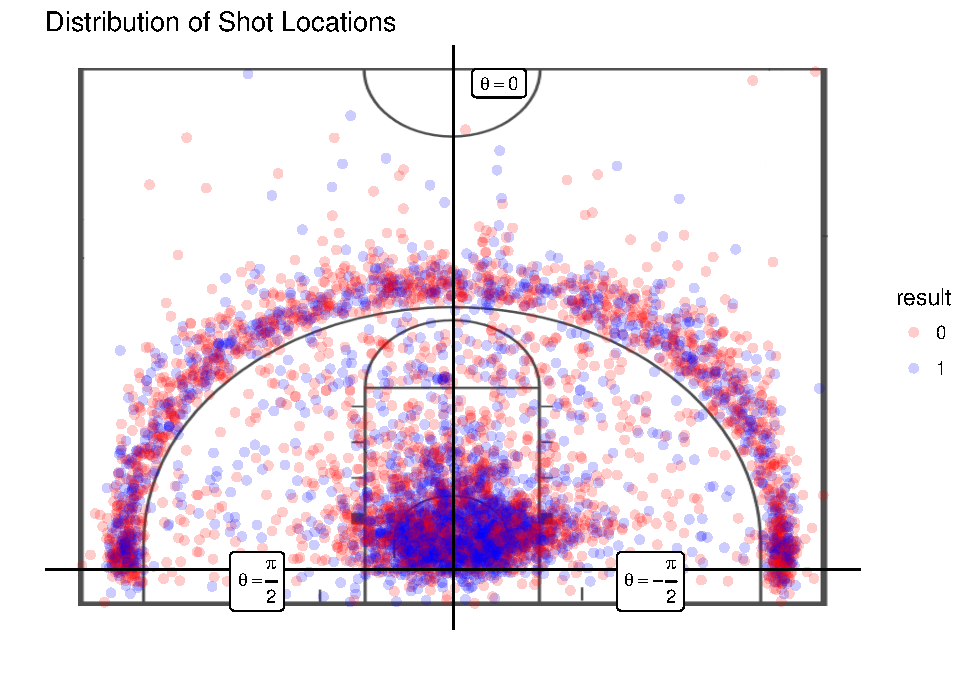
\includegraphics{thesis_files/figure-latex/shotplot-1.pdf}
\caption{\label{fig:shotplot}Locations and Results of All Shots}
\end{figure}
\section{Exploratory Data Analysis}\label{exploratory-data-analysis}

The following exploratory plots in Figure \ref{fig:smoothplot} examine
how consistent the probability of a made shot is, using a loess smooth
curve on the binary outcomes. We present these smoothed plots for four
high-usage basketball players at Duke University between the 2013-2014
and 2016-2017 seasons. Each plot represents a single player's ordered
shooting outcomes for a single season. These plots do not account for
the amount of time in between shots, but simply shot order and outcome.

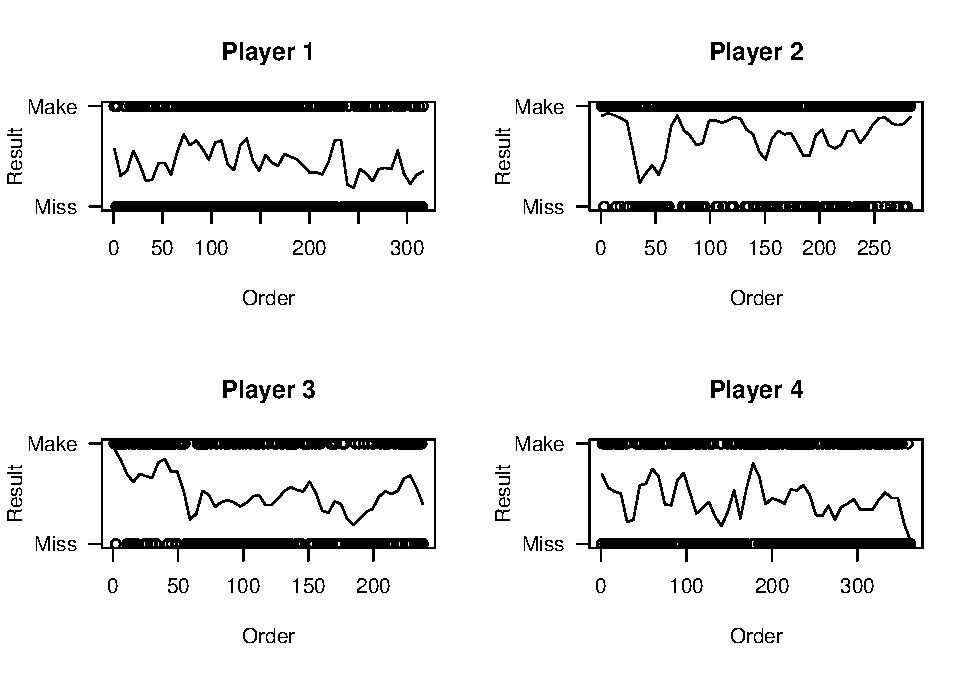
\includegraphics{thesis_files/figure-latex/smoothplot0-1.pdf}
\begin{figure}[htbp]
\centering
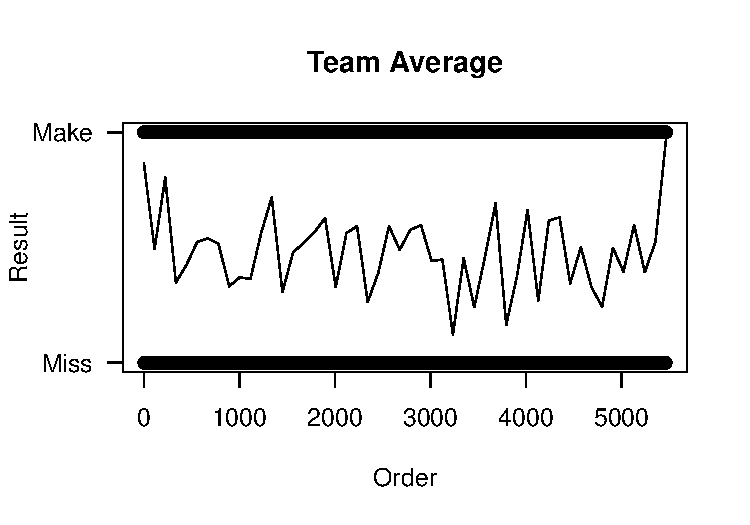
\includegraphics{thesis_files/figure-latex/smoothplot-1.pdf}
\caption{\label{fig:smoothplot}Moving Average of Shot Success Rate}
\end{figure}
We can see that the plots vary in the consistency of their made shots,
since they all contain spikes and trends. For example, the third plot
initially has a very high success rate, which quickly falls to the
middle after about thirty shot attempts, and the second plot has a
noticeable upward trend in shot success beginning around shot number one
hundred fifty.

We investigate the shooting outcomes using Bayesian models, and present
the results in the next section.

\chapter{Models \& Analysis}\label{models}

\section{Description of Models}\label{description-of-models}

For our models, we consider the shot location, the shooter identity, a
home court indicator, and a player's shooting success rate in nearby
games as factors that can affect a shot outcome. In every model, we use
the Just Another Gibbs Sampler library in R (\texttt{R2jags}). Each
model is based off of a logistic regression model that provides the
posterior distribution of the shot location parameters (distance and
angle). The models do not account for covariance between these
predictors. We expand upon this model by adding mixed effects and
discounted likelihood models to control for shooter identity and game
identity, respectively. These models will show us how consistent the
shot location parameters are between shooters and between games. In our
Gibbs Samplers, we estimate the posterior distributions using 10,000
simulations and a burn-in of 500. Our priors are made from the
corresponding Maximum Likelihood Estimates for the first four games in
the dataset, and we initialize our Monte Carlo Markov Chains using
values of 0 for all means, and 1 for all variances.

The \texttt{R2jags} code used to build these models, as well as some
diagnostic plots, can be found in Appendices \textbf{number} and
\textbf{number}, respectively.

\subsection{Generalized Linear Model}\label{generalized-linear-model}

First, we build a logistic regression model of the following form:

\[
\text{log} \left( \frac{p}{1-p} \right) = 
\beta_{\text{int}} +
x_{\text{r}}\beta_{\text{r}} +
x_{\theta}\beta_{\theta} +
x_{\text{H}}\beta_{\text{H}}.
\]

In this model, the \(x\) refers to the data, and the \(\beta\)s are the
pareters from the model. The subscripts \(\textit{int}\),
\(\textit{r}\), \(\theta\), and \(\textit{H}\) respectively refer to the
intercept, the log-distance of the shot, the angle of the shot, and
whether shot was taken on Duke's home court or another gym.

\subsection{Hierarchical Generalized Linear
Model}\label{hierarchical-generalized-linear-model}

Our second model is a hierarchical model, with random effects on the
\(\textit{j}\) players in the dataset. These random effects occur for
each of the four parameters of interest---the intercept, the home
effect, the distance effect, and the angle effect. Each individual
player's parameter values are sampled from a Normal distribution
centered at the population values. The parameters for players without a
lot of shot attemps are shrunk towards the population means.

\[
\text{log} \left( \frac{p}{1-p} \right) = 
\beta_{\text{int, j}} +
x_{\text{r}}\beta_{\text{r, j}} +
x_{\theta}\beta_{\theta, j} +
x_{\text{H}}\beta_{\text{H, j}},
\] \[
\beta_{\text{int, j}} \sim N(\beta_{\text{int}}, \tau^2_{\text{int}}),
\] \[
\beta_{\text{r, j}} \sim N(\beta_{\text{r}}, \tau^2_{\text{r}}),
\] \[
\beta_{\theta, j} \sim N(\beta_{\theta}, \tau^2_{\theta}),
\] \[
\beta_{\text{H, j}} \sim N(\beta_{\text{H}}, \tau^2_{\text{H}}).
\]

\subsection{Discounted Likelihood Hierarchical
Model}\label{discounted-likelihood-hierarchical-model}

In the discounted likelihood models, the likelihood of a single
observation at time \(\textit{t}\) is more heavily influenced by the
observations close to it than the observations far away from it. We
measure the ``distance'' between observations by the number of games
between them; a shot attempt that occurs in the next or the preceding
game will influence the likelihood of the observation more than a shot
that occurs two games away. To conceptualize this model, we first start
with a Forward Filtering model that uses a discounted Bayes Theorem. The
discounted Bayes Theorem, like the traditional Bayes Theorem, states
that the posterior is proportional to the product of the likelihood and
the prior, but it weights the most recent data higher than the earlier
data, which is weighted higher than the prior.

In other words, given the parameters: \[
\Theta = (\beta_{\text{int}}, \beta_{\text{r}}, \beta_{\theta}, \beta_\text{H}, \tau^2_{\text{int}}, \tau^2_{\text{r}}, \tau^2_{\theta})
\] the joint posterior distribution of the parameters given the data up
to time unit \(\textit{t}\), \(X_t\), is: \[
P_{g_t}(\Theta | X_t) \propto 
P(\Theta)^{\delta^t}
P(X_1|\Theta)^{\delta^{t-1}}
P(X_2|\Theta)^{\delta^{t-2}}...
P(X_{t-2}|\Theta)^{\delta^2}
P(X_{t-1}|\Theta)^{\delta}
P(X_t|\Theta)
\] \[
0 < \delta < 1
\] This equation shows that as distance from time \(\textit{t}\)
increases, the effect on the posterior distribution decreases. The
Reverse Updating extension of this concept allows the effect to take
place as the distance from \(\textit{t}\) increases in either the
positive or negative direction. \[
P_{g_t}(\Theta | X_t) \propto 
P(\Theta)^{\delta^t}...
P(X_{t-2}|\Theta)^{\delta^2}
P(X_{t-1}|\Theta)^{\delta}
P(X_t|\Theta)
P(X_{t+1}|\Theta)^{\delta}
P(X_{t+2}|\Theta)^{\delta^2}...
\] Specifically for our model, given an observed shot \(\textit{i}\) in
game \(g_i\), attempted by player \(\textit{j}\), we use the above
concept to discount the probability of a made shot in the hierarchical
model. \[
\text{log} \left( \frac{p}{1-p} \right) = 
\beta_{\text{int, j}} +
x_{\text{r}}\beta_{\text{r, j}} +
x_{\theta}\beta_{\theta, j} +
x_{\text{H}}\beta_{\text{H, j}},
\] \[
L(p) = 
\Pi_{\text{i=1}}^\text{n}p^{\text{y}_i} (1 - p)^{1-\text{y}_i},
\] \[
\delta_i = \Delta^{|g_i - g_t|},
\]

\[
\pi = L(p)^{\delta_i},
\] \[
\beta_{\text{int, j}} \sim N(\beta_{\text{int}}, \tau^2_{\text{int}}),
\] \[
\beta_{\text{r, j}} \sim N(\beta_{\text{r}}, \tau^2_{\text{r}}),
\] \[
\beta_{\theta, j} \sim N(\beta_{\theta}, \tau^2_{\theta}),
\] \[
\beta_{\text{H, j}} \sim N(\beta_{\text{H}}, \tau^2_{\text{H}}).
\] In this model, \(p\) represents the binomial likelihood, and \(\pi\)
is the discounted likelihood. Both of these quantities are probabilities
that are bounded in the interval {[}0,1{]}. The contribution of shot
outcomes (in the ``anchor game'' \(g_t\)) to the likelihood of the
current shot outcome (in game \(g_i\)) decreases as the distance between
the observations increases, and as \(\Delta\) decreases. In a model with
\(\Delta\) = 0, only shots taken in the same game as \(g_i\) can
contribute to the likelihood, while \(\Delta\) = 1 is equivalent to a
model with no discounting. If models with larger values of \(\Delta\)
best fit the data, this suggests that shooting success is consistent
throughout a career. If smaller values of \(\Delta\) are more likely in
the data, however, then we can assume there is a substantial amount of
time variation, or ``streakinss'' in the data on the game level. This
model specification results in an MCMC chain for each combination of
\(g_t\) and \(\Delta\). Figure \ref{fig:discplot} illustrates how the
likelihood weight of \(\delta\) depends on the selected value of
\(\Delta\) and the distance from the anchor game (\(|g_i - g_t|\)).
\begin{figure}[htbp]
\centering
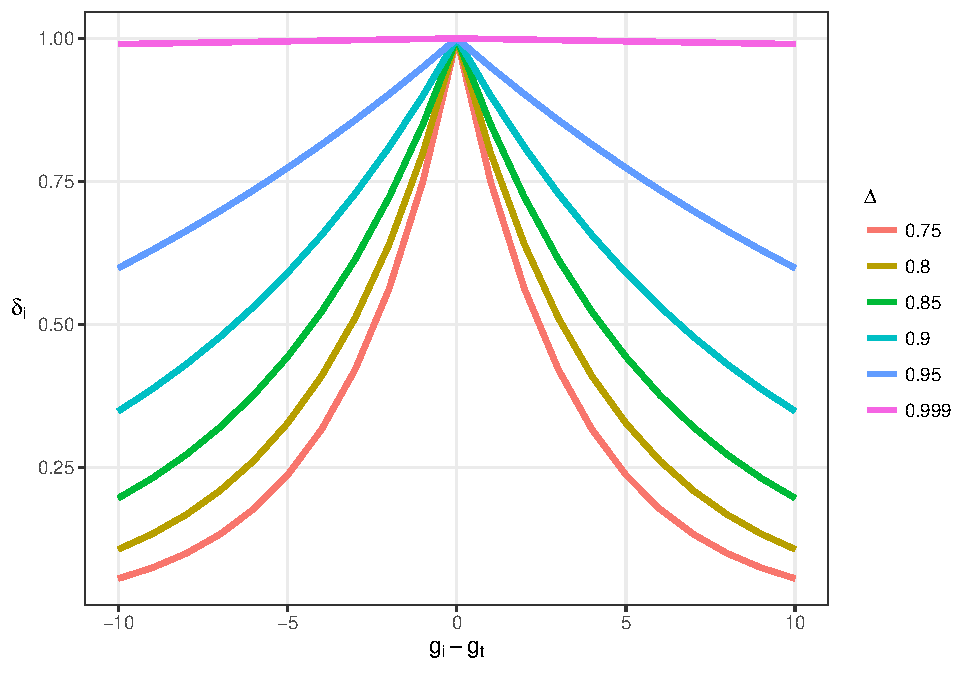
\includegraphics{thesis_files/figure-latex/discplot-1.pdf}
\caption{\label{fig:discplot}Illustration of Discounted Weighting}
\end{figure}
To build these discounted likelihood models in the \texttt{R2jags}
library, we apply the ``ones trick''. This technique allows us to do a
sampling distribution that do not exist in the library by modifying a
common distribution---in this case, the Binomial. The probability \(p\)
is estimated using the Bayesian hierarchical model. We discount this
probability to estimate \(\pi\), and then specify that artificial data
that consists only of ones comes from a Binomial distribution with the
discounted probability; this is equivalent to sampling from a
distribution with discounted outcomes. \textbf{elaborate on the ones
trick}. See Appendix \textbf{number} for the \texttt{R} code.

\section{Analysis}\label{analysis}

\subsection{Generalized Linear Model}\label{generalized-linear-model-1}

In our logistic regression model, we only look at shot location and the
home court indicator as predictors for the shot outcome. To look at
these effects for particular players, we simply subset the dataset to
shots attempted by that player before running the Gibbs Sampler. Below
in Figure \ref{fig:glmplot}, The 95\% credible intervals of the
posterior parameters are reported for the same four players that were
introduced in Figure \ref{fig:smoothplot}.

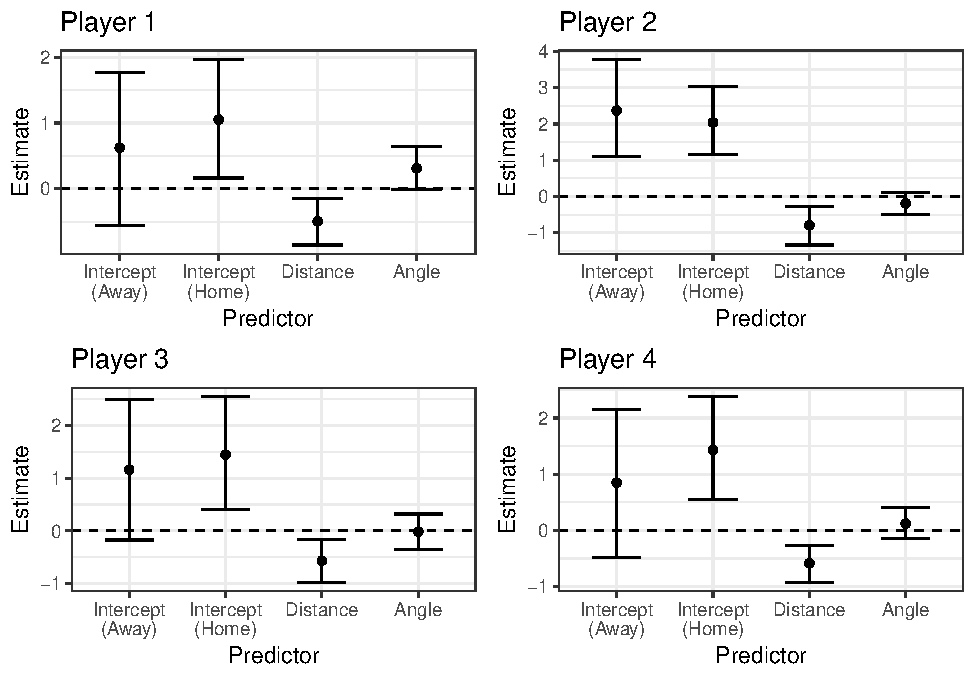
\includegraphics{thesis_files/figure-latex/glmplot0-1.pdf}
\begin{figure}

\hfill{}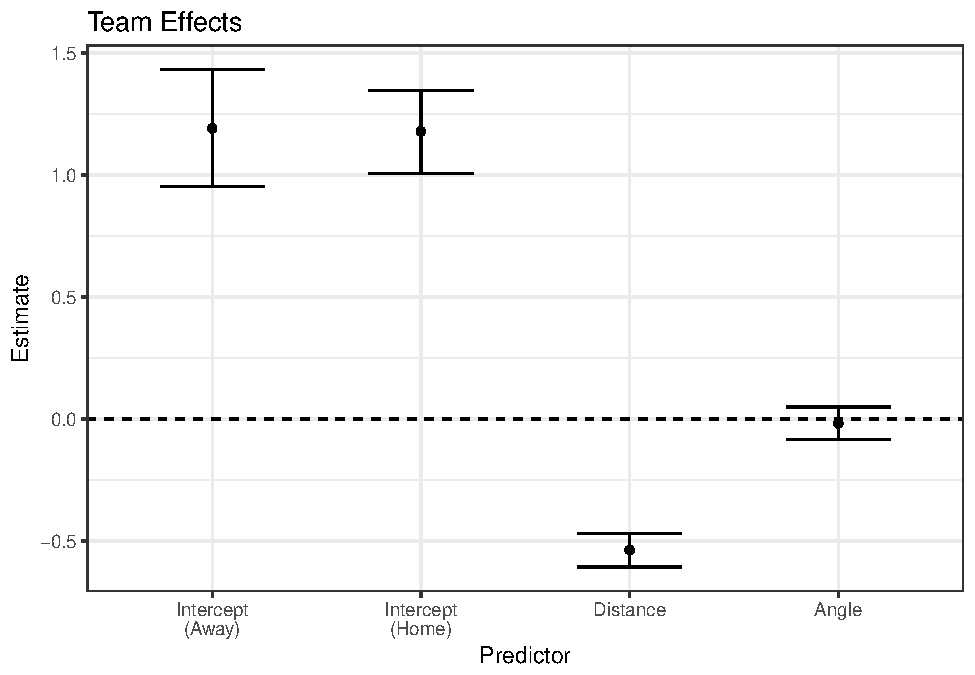
\includegraphics[width=0.9\linewidth]{thesis_files/figure-latex/glmplot-1} 

\caption{GLM Posterior Distributions for Four Players}\label{fig:glmplot}
\end{figure}
In the generalized linear model, the intercepts correspond to the
log-odds of making a shot when angle is zero (the middle of the court)
and the log distance is zero (one foot away from the hoop).

From these plots, we see that the team-wide 95\% credible interval of
the angle effect contains zero, and it is therefore probably not
predictive of a made shot. The average distance effect shows us that the
log-odds of a made shot decrease by \(\beta_r =\) 0.5372 as the log
distance increases by one unit and the other predictors remain constant.
In the probability scale, this decrease is:

\[
\frac{\text{e}^{\beta_r}}{1 + \text{e}^{\beta_r}} 
\]

which is equal to 0.3689.

We also see that the 95\% credible interval on the effect of distance is
completely negative, which follows the intuitive idea that the
probability of a made shot significantly decreases as distance from the
basket increases. The intercepts show us that there is not a substantial
diference in baseline shooting performance between home games and away
games.

\subsection{Hierarchical Generalized Linear
Model}\label{hierarchical-generalized-linear-model-1}

In this hierarchical model, we add random effects to allow the
parameters to vary for each player in the dataset. We present the
results below using densities of how the four players of interest
compare to the population distribution, and by using contour plots that
illustrate each player's probability of a made shot given their location
on the court for a game at home.
\begin{figure}[htbp]
\centering
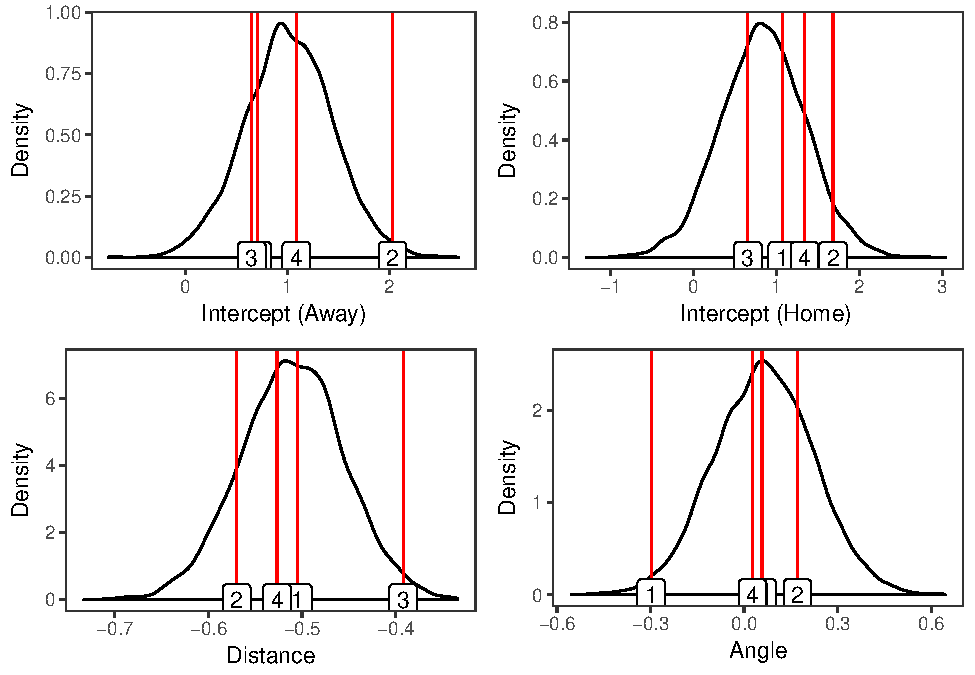
\includegraphics{thesis_files/figure-latex/hierplot-1.pdf}
\caption{\label{fig:hierplot}Population Distribution with Four Player
Effects}
\end{figure}
These hierarchical model results show us characteristics of our four
high-usage players of interest compared to the population of players in
the dataset. For example, the intercept plots show us that Player 2 is
excellent at finishing under baseline conditions, but he also has a
steeper-than-averge drop in his odds of scoring as his distance from the
basket increases. This means that most of his scoring occurs close to
the basket. We can also see that Player 1 strongly increases his odds of
scoring when his angle is negative, which corresponds to the left side
of the basket.

In the figures below, we have contour plots showing players' expected
field goal percentages at different locations on the court. Between our
four players of interest, we can observe how Player 1 is more effective
on the left side of the basket than the others, and how Player 2 has the
darkest overall contour plot, suggesting he has the highest probability
of scoring among those four.

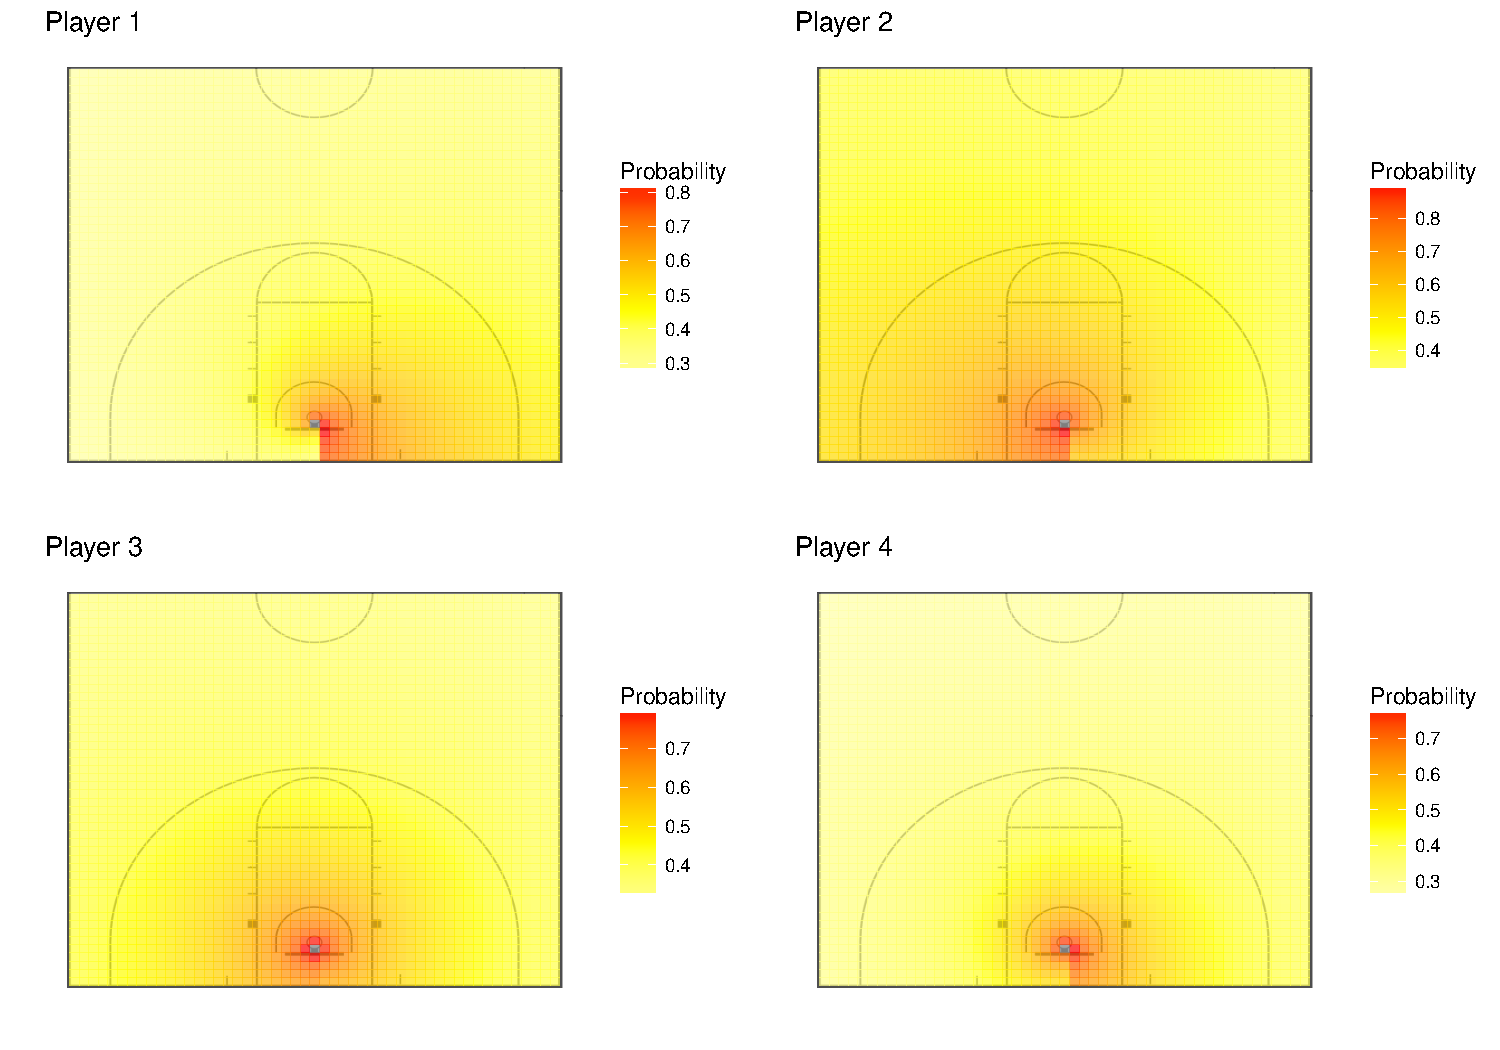
\includegraphics{thesis_files/figure-latex/contplot0-1.pdf}
\begin{figure}

\hfill{}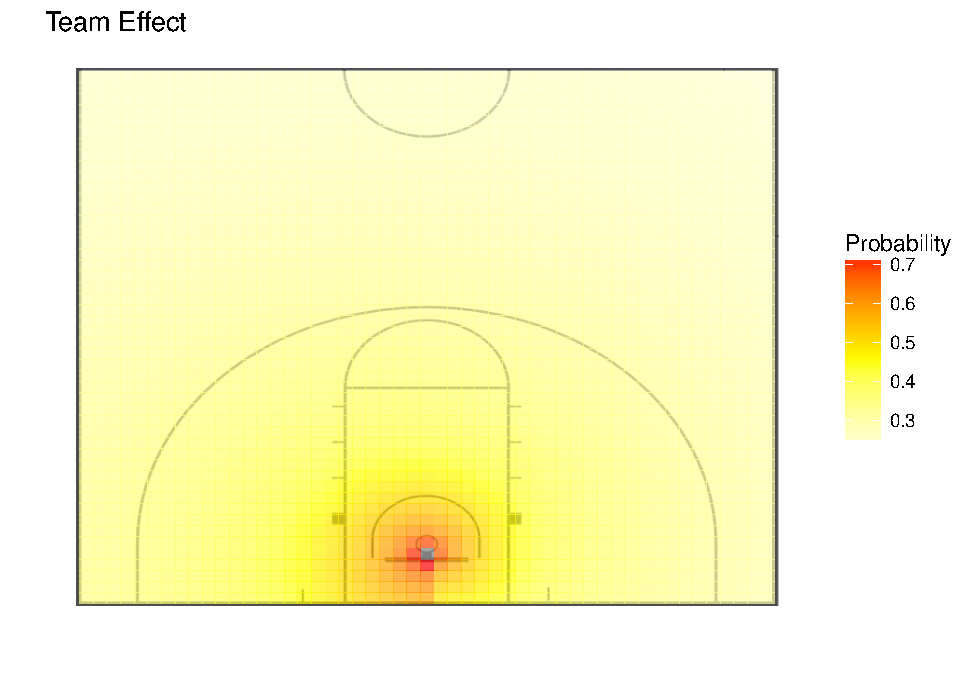
\includegraphics[width=0.9\linewidth]{thesis_files/figure-latex/contplot-1} 

\caption{Contour Plots for Four Players and Population of Players}\label{fig:contplot}
\end{figure}
\subsection{Discounted Likelihood Hierarchical
Model}\label{discounted-likelihood-hierarchical-model-1}

The values of \(\Delta\) that we use to fit the discounted likelihood
models are 0.750, 0.800, 0.850, 0.900, 0.950, and 0.999. We also build
an MCMC chain to estimate the posterior using every game as \(g_t\). We
calculate predictions and fitted values for a particular shot in game
\(g_i\) using the posterior median of the MCMC chain where \(g_i\) is
the anchor game \(g_t\).

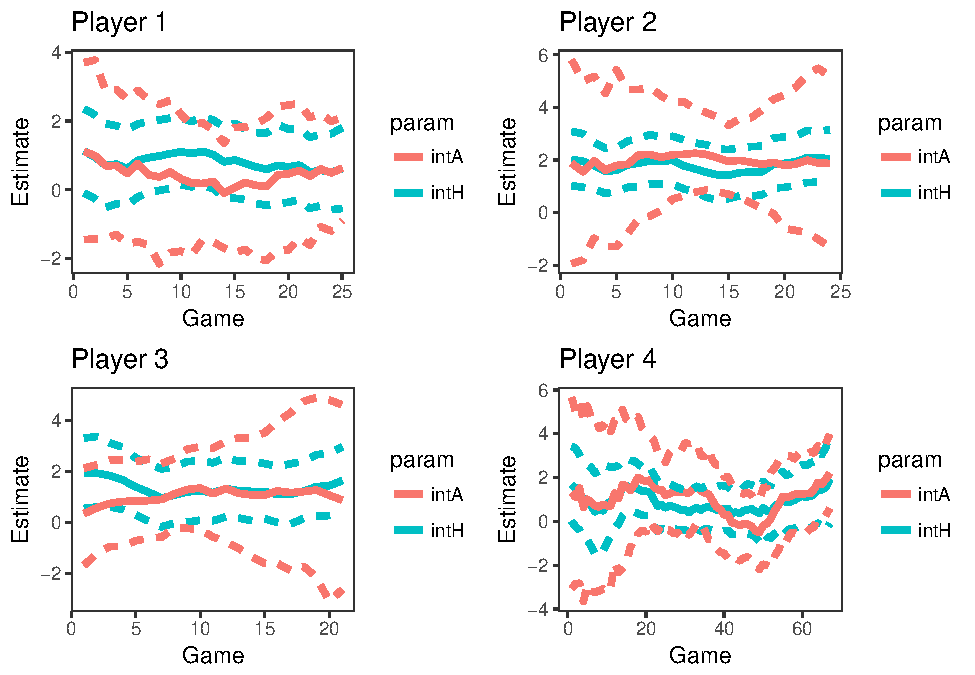
\includegraphics{thesis_files/figure-latex/discplot7500-1.pdf}
\begin{figure}

\hfill{}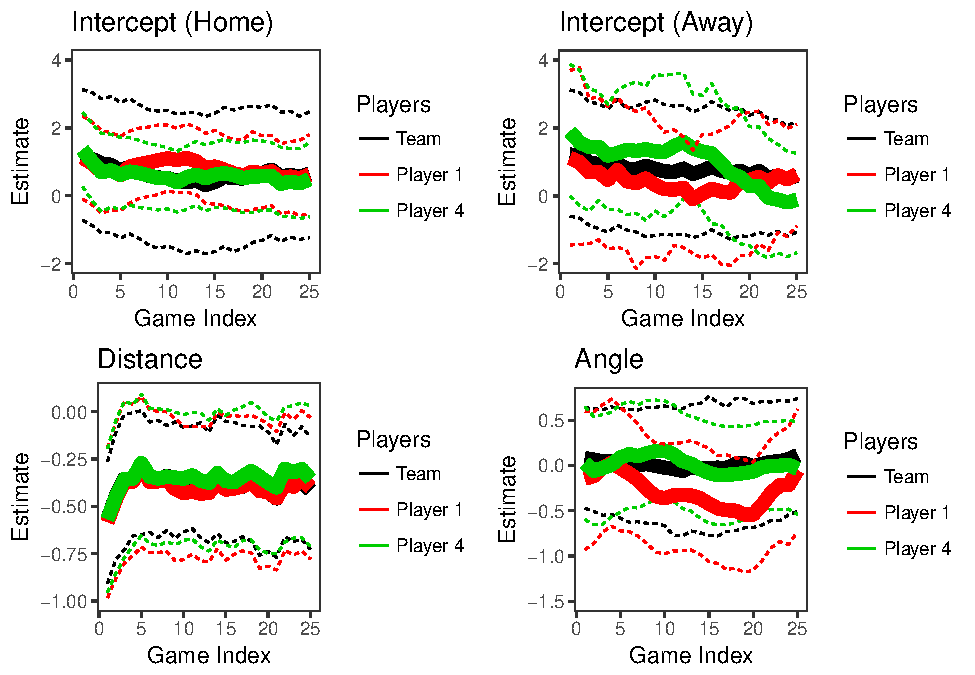
\includegraphics[width=0.9\linewidth]{thesis_files/figure-latex/discplot750-1} 

\caption{Intercepts for Four Players and Population over Time, $\Delta$ = 0.750}\label{fig:discplot750}
\end{figure}
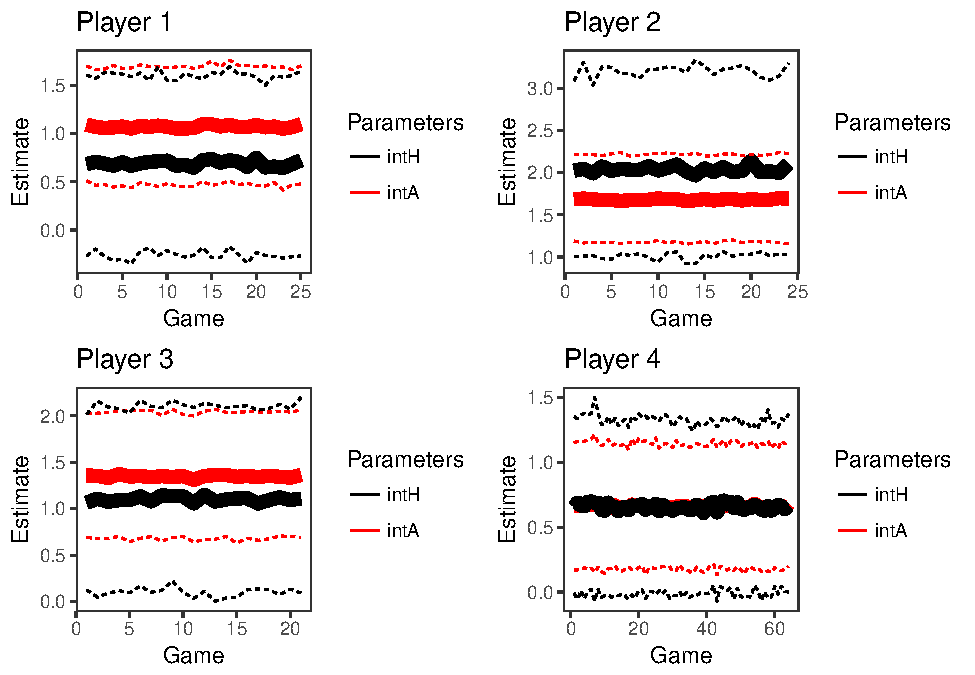
\includegraphics{thesis_files/figure-latex/discplot9990-1.pdf}
\begin{figure}

\hfill{}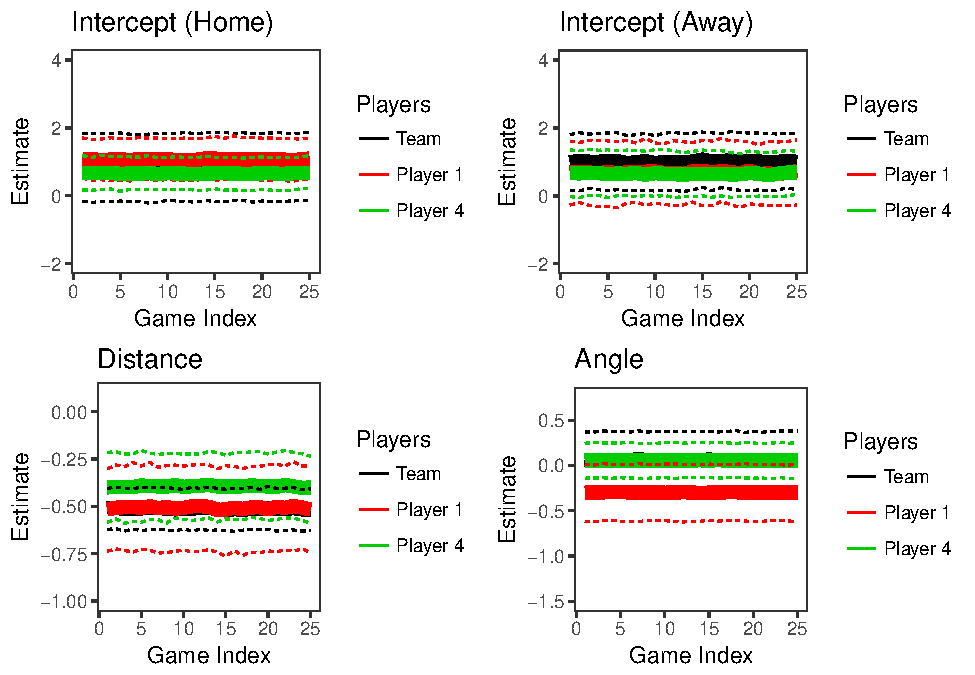
\includegraphics[width=0.9\linewidth]{thesis_files/figure-latex/discplot999-1} 

\caption{Intercepts for Four Players and Population over Time, $\Delta$ = 0.999}\label{fig:discplot999}
\end{figure}
The plots above illustrate how the intercepts change for the four
players and for the population over time. They also show how smaller
values of \(\Delta\) allow for greater variation in parameter values
over time.

\chapter{Discussion}\label{disc}

\section{Evaluation of Models}\label{evaluation-of-models}

To evaluate these models, we use 5-fold cross-validation. This process
used as many as 20 simultaneous RStudio Pro servers provided by the Duke
University Statistical Science Department. In each train-test split, we
evaluate a model's out-of-sample classification rate (using a cutoff
probability of 0.5), Brier score (mean squared error), and log
likelihood. The predictions and fitted values are obtained using MCMC
averages; to calculate the probability for an individual shot, we
calculate a response for each of the 9,500 posterior simulations, then
take the average of those responses. The results are plotted below:
\begin{figure}[htbp]
\centering
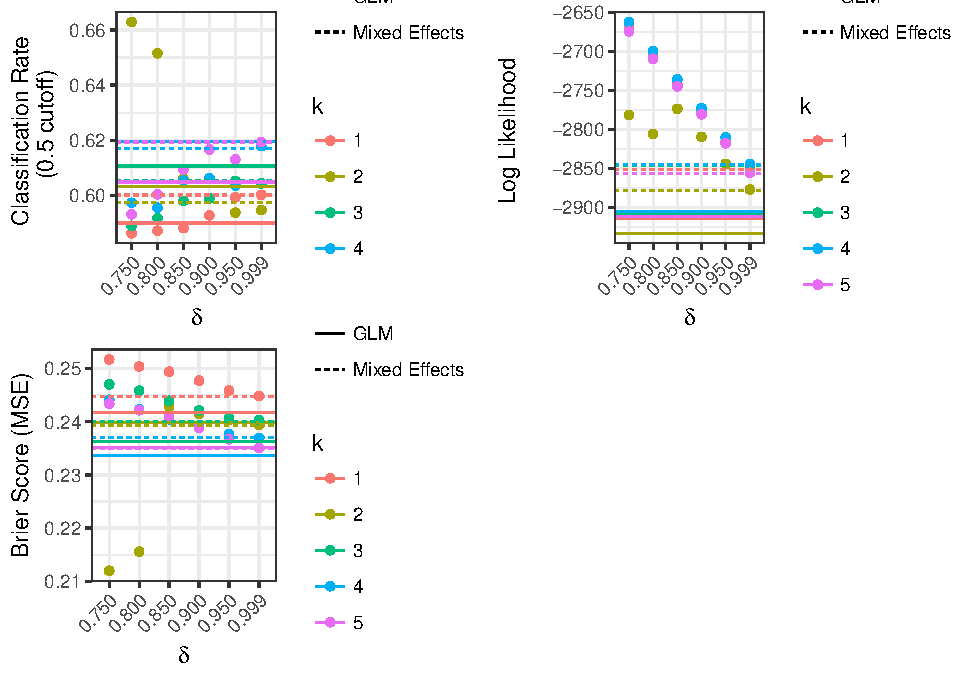
\includegraphics{thesis_files/figure-latex/evalplot-1.pdf}
\caption{\label{fig:evalplot}Model Evaluation}
\end{figure}
From Figure \ref{fig:evalplot}, we can observe that the models have
different strengths. The discounted likelihood model with the smallest
value of \(\Delta\) consistently has the highest likelihood. However, it
does not test as well as the other models in areas of out-of-sample
classification rate and Brier score. This suggests that models with
smaller values of \(\Delta\), where the likelihood of an observed shot
is more heavily influenced by shots closer to it, may overfit the model
to the training data. The generalized linear models perform best in
Brier score, but worst in log likelihood. The hierarchical models are
about the same, but they have a better log likelihood performance than
the GLMs. A model that balances the trade-off between predictive
accuracy and likelihood is a discounted likelihood model with \(\Delta\)
= 0.850.

In addition, we can see that the variation in model performance is
small. For example, most of the out-of-sample classification rates fall
between 0.58 and 0.62. This is within the 95\% confidence interval for a
random binomial proportion of 0.6 using a sample size of 40 (for each
combination of 5-fold cross-validation and 8 different models), which is
(0.5225, 0.6775). Therefore, the evidence that certain models predict
better than others is not particularly strong.

For the discounted likelihood model with \(\Delta\) = 0.850, we build
calibration plots to assess how well the estimated probabilities fit the
actual proportions. To make these plots, we divide the predicted
probabilities into 20 equally-sized bins, then plot these bins on the
x-axis versus the proportions of the actual outcomes within the bins on
the y-axis. The horizontal bars represent the bin width, and the
vertical bars represent a 95\% confidence interval of the proportions.
The red line of slope 1 represents equality between the bin medians and
the empirical probabilities within the bins. In Figure
\ref{fig:caliplot}, we present these plots for a full training set and a
testing set.
\begin{figure}[htbp]
\centering
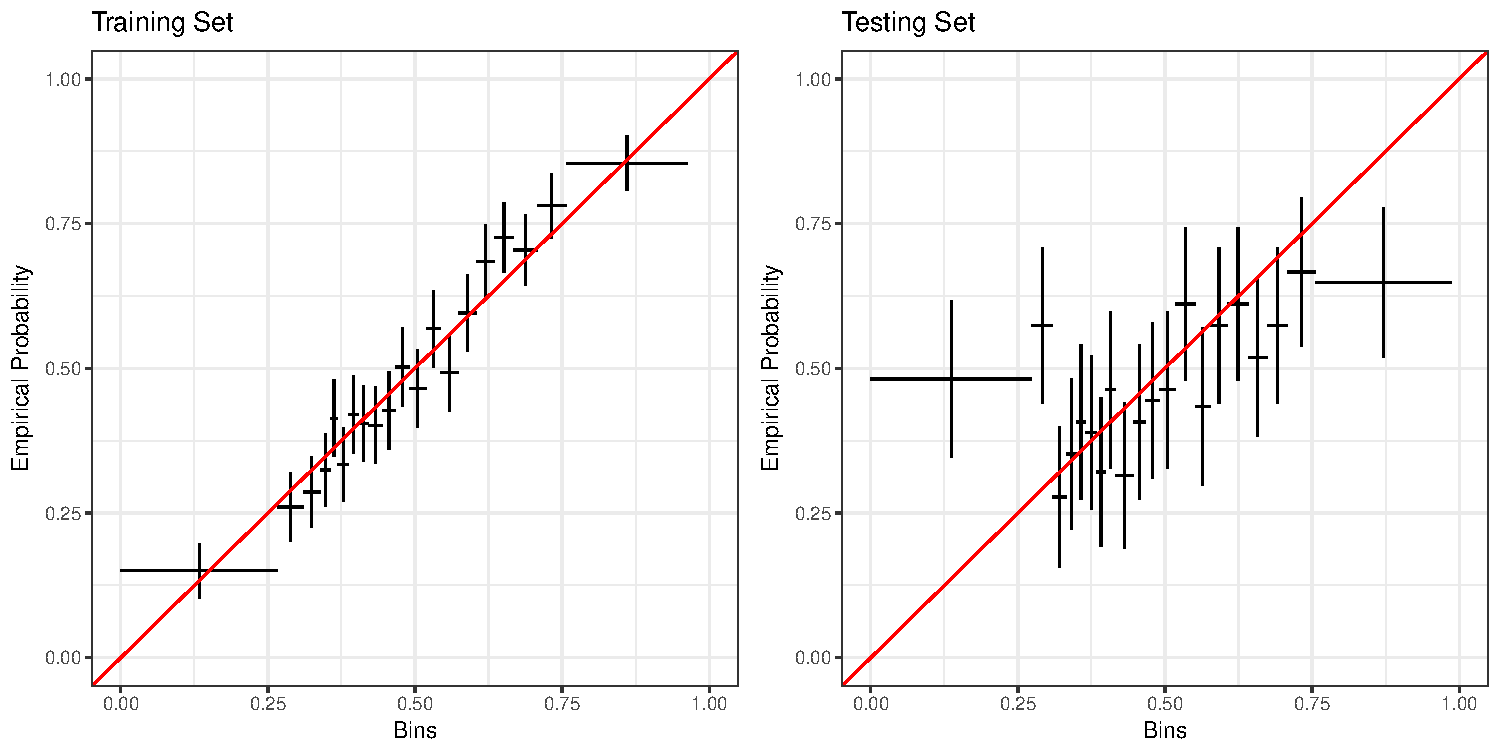
\includegraphics{thesis_files/figure-latex/caliplot-1.pdf}
\caption{\label{fig:caliplot}Calibration Plots for Discounted Likelihood
Model, \(\Delta\) = 0.850}
\end{figure}
In this model, we can see that the confidence intervals on the training
set all cross the line of slope, which shows that the model reliably
estimates the probabilities. In the testing set, however, the
predictions only cross this line between about 0.3 and 0.75. In
addition, the fact that the bins are so much thinner in the middle shows
that the model is not likely to predict values close to 0 or 1.

\section{Results from Model}\label{results-from-model}

To illustrate results from the discounted likelihood model with
\(\Delta\) = 0.850, we plot the location parameters over time for a
high-usage player and a low-usage player that play the same position,
and for the overall team. \textbf{make this sound more academic}

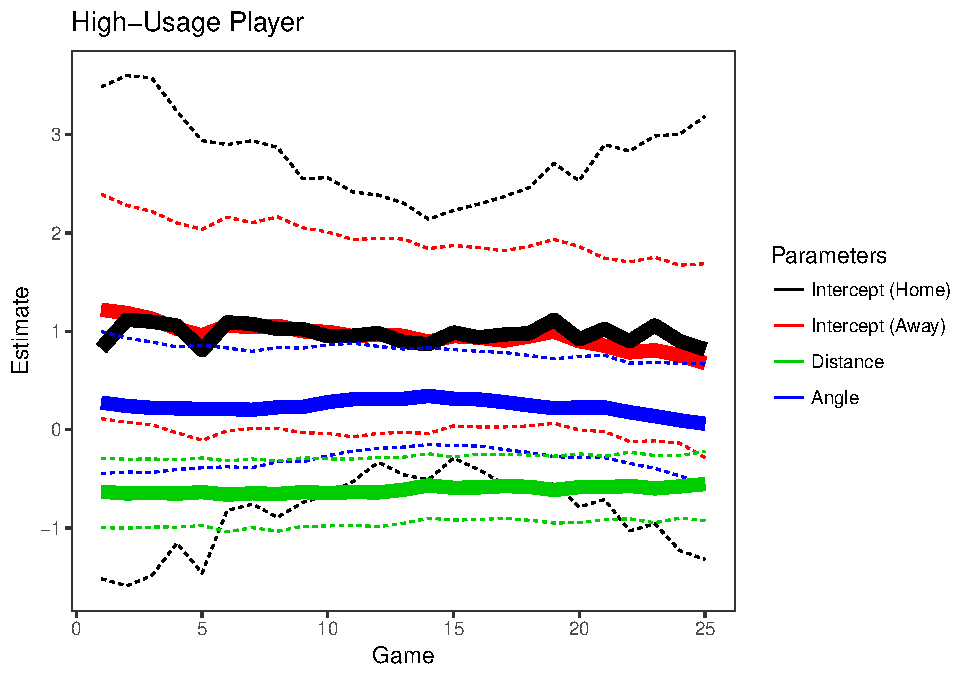
\includegraphics{thesis_files/figure-latex/discplot850-1.pdf}
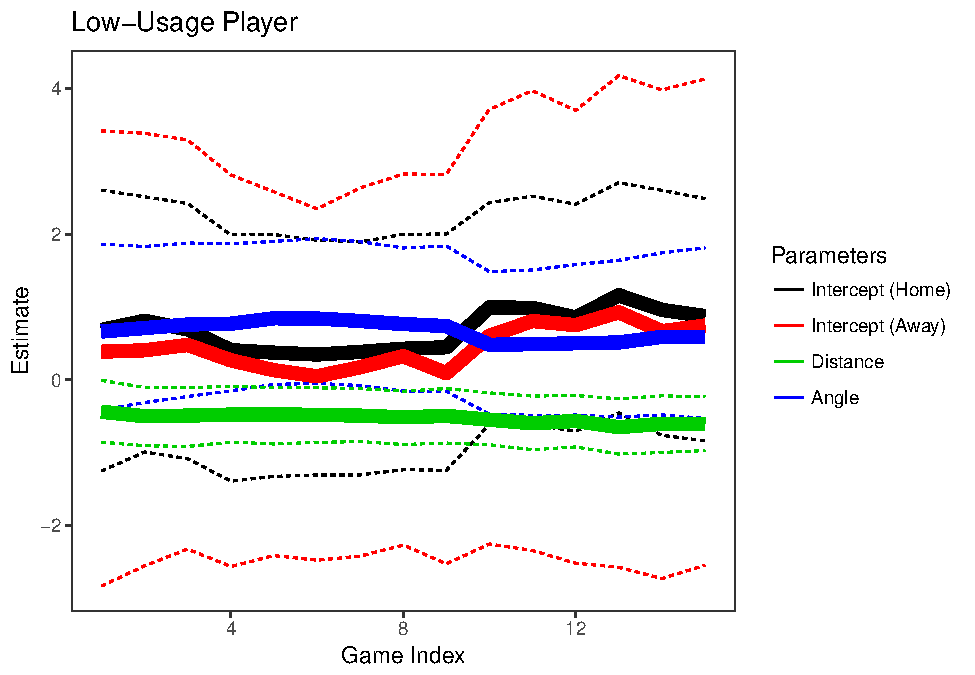
\includegraphics{thesis_files/figure-latex/discplot850-2.pdf}
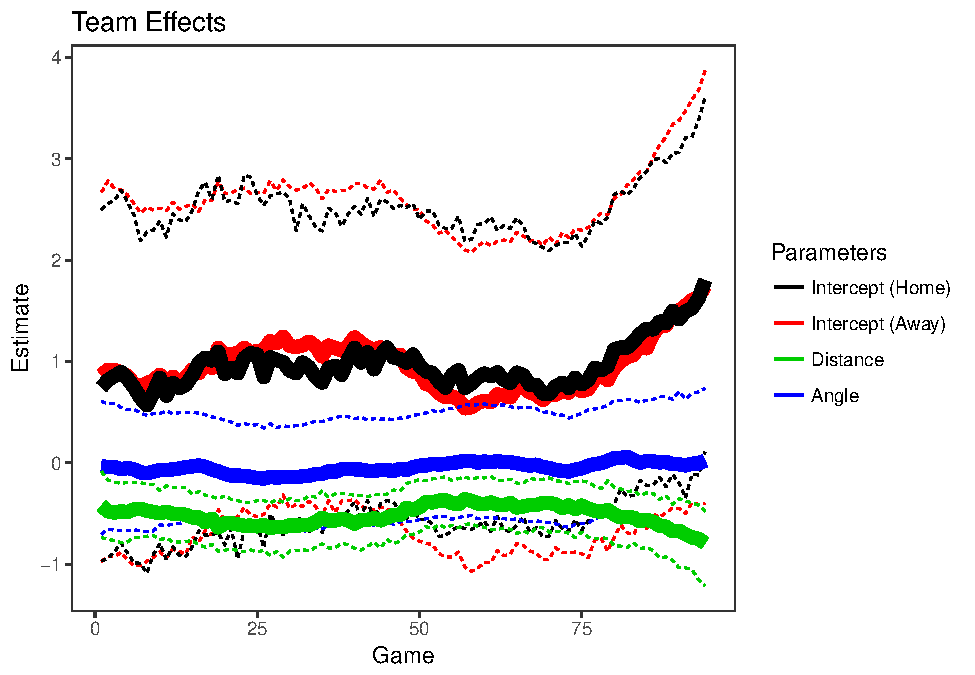
\includegraphics{thesis_files/figure-latex/discplot850-3.pdf}

We can see that the parameters move over time. \textbf{elaborate. like
the team parameters move the most over time. and the intercepts have
wider uncertainty.} The distance parameter moves the least. This
suggests that the ability to shoot long-range shots did not drastically
increase or decrease between games in the data.

\section{Conclusion}\label{conclusion}

The evaluations of the models show that there is not a lot of
time-dependency in shooting success rate in this dataset of
player-tracking data from the Duke Men's Basketball team. Allowing
predictors of shot success to shift based on recent success does not
significantly improve the predictive accuracy or the likelihood of a
model. However, we do see a systematic improvement in likelihood for
smaller discount factors (i.e., more emphasis on recent shots, and
therefore support of ``streakiness'').

To account for possible unexplained variation between seasons, and
variation introduced from having such a small population of road games,
I repeated this analysis on a subset of the data that only consisted of
shots from available games in the 2015 season (25 games), and shots from
home games (82 games). \textbf{results!} (show these results in
Appendix?)

\section{Future Goals}\label{future-goals}

Future goals for this research are to build a better-fitting model to
predict basketball shots using more advanced factors that can be
approximated from the dataset; possibilities for this include using the
distance of the nearest defender as a proxy for defense quality, or
using the amount of time a player has played without a substitution or
timeout to approximate fatigue.

\appendix

\chapter{Appendix 1: Code}\label{appendix-1-code}

\section{Generalized Linear Model}\label{generalized-linear-model-2}
\begin{Shaded}
\begin{Highlighting}[]
\NormalTok{Xtrainsub <-}\StringTok{ }
\StringTok{  }\NormalTok{Xtrain %>%}\StringTok{ }
\StringTok{  }\KeywordTok{filter}\NormalTok{(}\KeywordTok{as.integer}\NormalTok{(}\KeywordTok{as.factor}\NormalTok{(gameid)) <}\StringTok{ }\DecValTok{5}\NormalTok{)}

\NormalTok{priormod <-}\StringTok{ }\KeywordTok{glm}\NormalTok{(}\DataTypeTok{formula =} \NormalTok{result ~}\StringTok{ }\KeywordTok{log}\NormalTok{(r) +}\StringTok{ }\NormalTok{theta, }
                \DataTypeTok{data =} \NormalTok{Xtrainsub, }
                \DataTypeTok{family =} \StringTok{"binomial"}\NormalTok{)}

\NormalTok{mu0r <-}\StringTok{ }\KeywordTok{summary}\NormalTok{(priormod)[[}\StringTok{"coefficients"}\NormalTok{]][}\StringTok{"log(r)"}\NormalTok{,}\StringTok{"Estimate"}\NormalTok{]}
\NormalTok{mu0theta <-}\StringTok{ }\KeywordTok{summary}\NormalTok{(priormod)[[}\StringTok{"coefficients"}\NormalTok{]][}\StringTok{"theta"}\NormalTok{,}\StringTok{"Estimate"}\NormalTok{]}

\NormalTok{fit_glm <-}\StringTok{ }\NormalTok{function(dat, }\DataTypeTok{S =} \DecValTok{10000}\NormalTok{, }\DataTypeTok{B =} \DecValTok{500}\NormalTok{)\{}

  \NormalTok{model.glm <-}\StringTok{ }\NormalTok{function()\{}
  
    \CommentTok{# Liklihood function (for N observations)}
    \NormalTok{for(i in }\DecValTok{1}\NormalTok{:N)\{}
      
      \KeywordTok{logit}\NormalTok{(prob[i]) <-}\StringTok{ }\NormalTok{beta_int*int[i] +}\StringTok{ }
\StringTok{        }\NormalTok{beta_home*home[i] +}
\StringTok{        }\NormalTok{beta_r*logr[i] +}\StringTok{ }
\StringTok{        }\NormalTok{beta_theta*theta[i]}
      
      \NormalTok{result[i] ~}\StringTok{ }\KeywordTok{dbern}\NormalTok{(prob[i])}
    \NormalTok{\}}

    \CommentTok{# Priors}
    \CommentTok{# we expect less variation in the distance parameter, }
    \CommentTok{# because shot success rate should get worse }
    \CommentTok{# as distance increases under baseline circumstances.}
    \NormalTok{beta_int   ~}\StringTok{ }\KeywordTok{dnorm}\NormalTok{(}\DecValTok{0}\NormalTok{, }\FloatTok{0.1}\NormalTok{)}
    \NormalTok{beta_home  ~}\StringTok{ }\KeywordTok{dnorm}\NormalTok{(}\DecValTok{0}\NormalTok{, }\FloatTok{0.1}\NormalTok{)}
    \NormalTok{beta_r     ~}\StringTok{ }\KeywordTok{dnorm}\NormalTok{(mu0r, }\FloatTok{0.01}\NormalTok{) }
    \NormalTok{beta_theta ~}\StringTok{ }\KeywordTok{dnorm}\NormalTok{(mu0theta, }\FloatTok{0.1}\NormalTok{)}
  \NormalTok{\}}

  \NormalTok{datlist.glm <-}\StringTok{  }
\StringTok{    }\KeywordTok{list}\NormalTok{(}
      \DataTypeTok{int =} \KeywordTok{rep}\NormalTok{(}\DecValTok{1}\NormalTok{, }\KeywordTok{nrow}\NormalTok{(dat)),}
      \DataTypeTok{logr =} \KeywordTok{log}\NormalTok{(dat$r), }
      \DataTypeTok{theta =} \NormalTok{dat$theta, }
      \DataTypeTok{result =} \NormalTok{dat$result,}
      \DataTypeTok{home =} \NormalTok{dat$home,}
      \DataTypeTok{N =} \KeywordTok{nrow}\NormalTok{(dat), }
      \DataTypeTok{mu0r =} \NormalTok{mu0r,}
      \DataTypeTok{mu0theta =} \NormalTok{mu0theta}
    \NormalTok{)}
  
  \NormalTok{params.glm <-}\StringTok{ }\KeywordTok{c}\NormalTok{(}\StringTok{"beta_int"}\NormalTok{,}
                  \StringTok{"beta_home"}\NormalTok{,}
                  \StringTok{"beta_r"}\NormalTok{,}
                  \StringTok{"beta_theta"}\NormalTok{)}

  \NormalTok{initslist <-}\StringTok{ }\KeywordTok{list}\NormalTok{(}\KeywordTok{list}\NormalTok{(}\StringTok{"beta_int"}\NormalTok{=}\DecValTok{0}\NormalTok{, }
                         \StringTok{"beta_r"}\NormalTok{=}\DecValTok{0}\NormalTok{, }
                         \StringTok{"beta_theta"}\NormalTok{=}\DecValTok{0}\NormalTok{, }
                         \StringTok{"beta_home"}\NormalTok{=}\DecValTok{0}\NormalTok{))}
                    
  \NormalTok{sim <-}\StringTok{ }
\StringTok{    }\KeywordTok{jags}\NormalTok{(}\DataTypeTok{data =} \NormalTok{datlist.glm, }
         \DataTypeTok{n.chains =} \DecValTok{1}\NormalTok{, }\DataTypeTok{n.iter =} \NormalTok{S, }\DataTypeTok{n.burnin =} \NormalTok{B, }\DataTypeTok{n.thin =} \DecValTok{1}\NormalTok{,}
         \DataTypeTok{inits=}\NormalTok{initslist,}
         \DataTypeTok{parameters.to.save =} \NormalTok{params.glm,}
         \DataTypeTok{model.file=}\NormalTok{model.glm}
    \NormalTok{)}
  
  \NormalTok{sim.mcmc <-}\StringTok{ }\KeywordTok{as.data.frame}\NormalTok{(}\KeywordTok{as.mcmc}\NormalTok{(sim)[[}\DecValTok{1}\NormalTok{]])}
  
  \CommentTok{# Changing from a baseline mean + a shift amount}
  \CommentTok{# to two different means based on the type of game.}
  \NormalTok{sim.mcmc <-}\StringTok{ }
\StringTok{    }\NormalTok{sim.mcmc %>%}\StringTok{ }
\StringTok{    }\KeywordTok{mutate}\NormalTok{(}\DataTypeTok{beta_intA =} \NormalTok{beta_int,}
           \DataTypeTok{beta_intH =} \NormalTok{beta_int +}\StringTok{ }\NormalTok{beta_home) %>%}
\StringTok{    }\KeywordTok{select}\NormalTok{(beta_intA, beta_intH, beta_r, beta_theta)}
  
  \KeywordTok{return}\NormalTok{(sim.mcmc)}
\NormalTok{\}}
\end{Highlighting}
\end{Shaded}
\section{Hierarchical Generalized Linear
Model}\label{hierarchical-generalized-linear-model-2}
\begin{Shaded}
\begin{Highlighting}[]
\NormalTok{Xtrainsub <-}\StringTok{ }
\StringTok{  }\NormalTok{Xtrain %>%}\StringTok{ }
\StringTok{  }\KeywordTok{filter}\NormalTok{(}\KeywordTok{as.integer}\NormalTok{(}\KeywordTok{as.factor}\NormalTok{(gameid)) <}\StringTok{ }\DecValTok{5}\NormalTok{)}

\NormalTok{priormod <-}\StringTok{ }\KeywordTok{glm}\NormalTok{(}\DataTypeTok{formula =} \NormalTok{result ~}\StringTok{ }\KeywordTok{log}\NormalTok{(r) +}\StringTok{ }\NormalTok{theta, }
                \DataTypeTok{data =} \NormalTok{Xtrainsub, }
                \DataTypeTok{family =} \StringTok{"binomial"}\NormalTok{)}

\NormalTok{mu0r <-}\StringTok{ }\KeywordTok{summary}\NormalTok{(priormod)[[}\StringTok{"coefficients"}\NormalTok{]][}\StringTok{"log(r)"}\NormalTok{,}\StringTok{"Estimate"}\NormalTok{]}
\NormalTok{mu0theta <-}\StringTok{ }\KeywordTok{summary}\NormalTok{(priormod)[[}\StringTok{"coefficients"}\NormalTok{]][}\StringTok{"theta"}\NormalTok{,}\StringTok{"Estimate"}\NormalTok{]}

\NormalTok{fit_players <-}\StringTok{ }\NormalTok{function(}\DataTypeTok{dat =} \OtherTok{NA}\NormalTok{, }\DataTypeTok{S =} \DecValTok{10000}\NormalTok{, }\DataTypeTok{B =} \DecValTok{500}\NormalTok{)\{}
  
  \NormalTok{model.player <-}\StringTok{ }\NormalTok{function()\{}
    
    \CommentTok{# Likelihood function for N observations}
    \NormalTok{for(i in }\DecValTok{1}\NormalTok{:N)\{}
      
      \CommentTok{# the parameters now vary by player id.}
      \KeywordTok{logit}\NormalTok{(prob[i]) <-}\StringTok{ }\NormalTok{beta_int[player[i]]*int[i] +}\StringTok{ }
\StringTok{        }\NormalTok{beta_home[player[i]]*home[i] +}\StringTok{ }
\StringTok{        }\NormalTok{beta_r[player[i]]*logr[i] +}\StringTok{ }
\StringTok{        }\NormalTok{beta_theta[player[i]]*theta[i]}
      
      \NormalTok{result[i] ~}\StringTok{ }\KeywordTok{dbern}\NormalTok{(prob[i])}
    \NormalTok{\}}
    
    \CommentTok{# Priors}
    \NormalTok{for(j in }\DecValTok{1}\NormalTok{:M)\{}
        \NormalTok{beta_int[j] ~}\StringTok{ }\KeywordTok{dnorm}\NormalTok{(beta_int0,tau_int)}
        \NormalTok{beta_home[j]  ~}\StringTok{ }\KeywordTok{dnorm}\NormalTok{(beta_home0, tau_int)}
        \NormalTok{beta_r[j] ~}\StringTok{ }\KeywordTok{dnorm}\NormalTok{(beta_r0,tau_r)}
        \NormalTok{beta_theta[j] ~}\StringTok{ }\KeywordTok{dnorm}\NormalTok{(beta_theta0,tau_theta)}
    \NormalTok{\}}
    
    \CommentTok{# Hyperpriors}
    \NormalTok{beta_int0   ~}\StringTok{ }\KeywordTok{dnorm}\NormalTok{(}\DecValTok{0}\NormalTok{, }\FloatTok{0.1}\NormalTok{)}
    \NormalTok{beta_home0  ~}\StringTok{ }\KeywordTok{dnorm}\NormalTok{(}\DecValTok{0}\NormalTok{, }\FloatTok{0.1}\NormalTok{)}
    \NormalTok{beta_r0     ~}\StringTok{ }\KeywordTok{dnorm}\NormalTok{(mu0r, }\FloatTok{0.01}\NormalTok{)}
    \NormalTok{beta_theta0 ~}\StringTok{ }\KeywordTok{dnorm}\NormalTok{(mu0theta, }\FloatTok{0.1}\NormalTok{)}
    \NormalTok{tau_int ~}\StringTok{ }\KeywordTok{dgamma}\NormalTok{(}\DecValTok{10}\NormalTok{, }\DecValTok{100}\NormalTok{)}
    \NormalTok{tau_r ~}\StringTok{ }\KeywordTok{dgamma}\NormalTok{(}\DecValTok{10}\NormalTok{, }\FloatTok{0.2}\NormalTok{)}
    \NormalTok{tau_theta ~}\StringTok{ }\KeywordTok{dgamma}\NormalTok{(}\DecValTok{10}\NormalTok{, }\DecValTok{10}\NormalTok{)}
  \NormalTok{\}}

  \NormalTok{datlist.player <-}\StringTok{ }
\StringTok{    }\KeywordTok{list}\NormalTok{(}
      \DataTypeTok{logr =} \KeywordTok{log}\NormalTok{(dat$r), }
      \DataTypeTok{theta =} \NormalTok{dat$theta, }
      \DataTypeTok{home =} \NormalTok{dat$home,}
      \DataTypeTok{result =} \NormalTok{dat$result, }
      \DataTypeTok{player =} \KeywordTok{as.integer}\NormalTok{(}\KeywordTok{as.factor}\NormalTok{(dat$globalplayerid)),}
      \DataTypeTok{N =} \KeywordTok{nrow}\NormalTok{(dat), }
      \DataTypeTok{int =} \KeywordTok{rep}\NormalTok{(}\DecValTok{1}\NormalTok{, }\KeywordTok{nrow}\NormalTok{(dat)), }
      \DataTypeTok{M =} \KeywordTok{n_distinct}\NormalTok{(dat$globalplayerid),}
      \DataTypeTok{mu0r =} \NormalTok{mu0r,}
      \DataTypeTok{mu0theta =} \NormalTok{mu0theta}
    \NormalTok{)}
  
  \CommentTok{# we want posteriors for the overall effects }
  \CommentTok{# and for the individual player effects}
  \NormalTok{params <-}\StringTok{ }\KeywordTok{c}\NormalTok{(}\StringTok{"beta_int"}\NormalTok{, }
              \StringTok{"beta_home"}\NormalTok{, }
              \StringTok{"beta_r"}\NormalTok{, }
              \StringTok{"beta_theta"}\NormalTok{,}
              \StringTok{"beta_int0"}\NormalTok{,}
              \StringTok{"beta_home0"}\NormalTok{,}
              \StringTok{"beta_r0"}\NormalTok{, }
              \StringTok{"beta_theta0"}\NormalTok{)}

  \NormalTok{M <-}\StringTok{ }\NormalTok{datlist.player$M}
  
  \NormalTok{initslist <-}\StringTok{ }\KeywordTok{list}\NormalTok{(}
    \KeywordTok{list}\NormalTok{(}\StringTok{"beta_int"}\NormalTok{=}\KeywordTok{rep}\NormalTok{(}\DecValTok{0}\NormalTok{,M), }
         \StringTok{"beta_home"}\NormalTok{=}\KeywordTok{rep}\NormalTok{(}\DecValTok{0}\NormalTok{,M), }
         \StringTok{"beta_r"}\NormalTok{=}\KeywordTok{rep}\NormalTok{(}\DecValTok{0}\NormalTok{,M), }
         \StringTok{"beta_theta"}\NormalTok{=}\KeywordTok{rep}\NormalTok{(}\DecValTok{0}\NormalTok{,M),}
         \StringTok{"beta_int0"}\NormalTok{=}\DecValTok{0}\NormalTok{,}
         \StringTok{"beta_home0"}\NormalTok{=}\DecValTok{0}\NormalTok{,}
         \StringTok{"beta_r0"}\NormalTok{=}\DecValTok{0}\NormalTok{, }
         \StringTok{"beta_theta0"}\NormalTok{=}\DecValTok{0}\NormalTok{, }
         \StringTok{"tau_int"}\NormalTok{=}\DecValTok{1}\NormalTok{, }
         \StringTok{"tau_r"}\NormalTok{=}\DecValTok{1}\NormalTok{, }
         \StringTok{"tau_theta"}\NormalTok{=}\DecValTok{1}
  \NormalTok{))}

  \NormalTok{sim.player <-}\StringTok{ }
\StringTok{    }\KeywordTok{jags}\NormalTok{(}\DataTypeTok{data =} \NormalTok{datlist.player, }
         \DataTypeTok{n.iter =} \NormalTok{S, }\DataTypeTok{n.chains =} \DecValTok{1}\NormalTok{, }\DataTypeTok{n.burnin =} \NormalTok{B, }\DataTypeTok{n.thin =} \DecValTok{1}\NormalTok{,}
         \DataTypeTok{inits=}\NormalTok{initslist,}
         \DataTypeTok{parameters.to.save =} \NormalTok{params,}
         \DataTypeTok{model.file=}\NormalTok{model.player}
  \NormalTok{)}
  
  \NormalTok{sim.mcmc.player <-}\StringTok{ }\KeywordTok{as.data.frame}\NormalTok{(}\KeywordTok{as.mcmc}\NormalTok{(sim.player)[[}\DecValTok{1}\NormalTok{]])}
  
  
  \CommentTok{# Changing from a baseline mean + a shift amount}
  \CommentTok{# to two different means based on the type of game.}
  \NormalTok{hometext <-}\StringTok{ }\KeywordTok{paste0}\NormalTok{(}\StringTok{"`beta_intH["}\NormalTok{,}\DecValTok{1}\NormalTok{:M,}\StringTok{"]` = }
\StringTok{                     `beta_int["}\NormalTok{,}\DecValTok{1}\NormalTok{:M,}\StringTok{"]` + }
\StringTok{                     `beta_home["}\NormalTok{,}\DecValTok{1}\NormalTok{:M,}\StringTok{"]`"}\NormalTok{,}
                     \DataTypeTok{collapse=}\StringTok{",}\CharTok{\textbackslash{}n}\StringTok{"}\NormalTok{)}
  
  \NormalTok{awaytext <-}\StringTok{ }\KeywordTok{paste0}\NormalTok{(}\StringTok{"`beta_intA["}\NormalTok{,}\DecValTok{1}\NormalTok{:M,}\StringTok{"]` = }
\StringTok{                     `beta_int["}\NormalTok{,}\DecValTok{1}\NormalTok{:M,}\StringTok{"]`"}\NormalTok{, }
                     \DataTypeTok{collapse=}\StringTok{",}\CharTok{\textbackslash{}n}\StringTok{"}\NormalTok{)}
  
  \NormalTok{sim.mcmc.player <-}\StringTok{ }\KeywordTok{eval}\NormalTok{(}\KeywordTok{parse}\NormalTok{(}\DataTypeTok{text=}
    \KeywordTok{paste0}\NormalTok{(}\StringTok{"sim.mcmc.player %>%}
\StringTok{              mutate("}\NormalTok{,hometext,}\StringTok{", beta_intH0 = beta_int0 + beta_home0)"}\NormalTok{,}\StringTok{" %>%}
\StringTok{              rename("}\NormalTok{,awaytext,}\StringTok{", beta_intA0 = beta_int0)"}
           \NormalTok{))) %>%}
\StringTok{    }\KeywordTok{select}\NormalTok{(}\KeywordTok{grep}\NormalTok{(}\StringTok{"(beta_int)|(beta_theta)|(beta_r)"}\NormalTok{,}\KeywordTok{names}\NormalTok{(.)))}
  
  \NormalTok{sim.mcmc.player <-}\StringTok{ }\NormalTok{sim.mcmc.player[ ,}\KeywordTok{order}\NormalTok{(}\KeywordTok{colnames}\NormalTok{(sim.mcmc.player))]}
  
  
  \CommentTok{# Renaming mixed effects columns from default factor levels (integers) to the corresponding player ids}
  
  \NormalTok{factorids <-}\StringTok{ }
\StringTok{    }\KeywordTok{str_extract_all}\NormalTok{(}\KeywordTok{names}\NormalTok{(sim.mcmc.player), }\StringTok{"[[:digit:]]+"}\NormalTok{) %>%}\StringTok{ }
\StringTok{    }\KeywordTok{as.numeric}\NormalTok{()}
  
  \NormalTok{fids <-}\StringTok{ }\KeywordTok{data.frame}\NormalTok{(}\DataTypeTok{factorid =} \NormalTok{factorids, }\DataTypeTok{order =} \DecValTok{1}\NormalTok{:}\KeywordTok{length}\NormalTok{(factorids))}
  
  \NormalTok{datmap <-}\StringTok{ }\NormalTok{dat %>%}\StringTok{ }
\StringTok{    }\KeywordTok{mutate}\NormalTok{(}\DataTypeTok{factorid =} \KeywordTok{as.integer}\NormalTok{(}\KeywordTok{as.factor}\NormalTok{(globalplayerid))) %>%}
\StringTok{    }\KeywordTok{select}\NormalTok{(globalplayerid, factorid)}
  
  \NormalTok{gameids <-}\StringTok{ }\KeywordTok{merge}\NormalTok{(datmap, fids, }\DataTypeTok{all.x=}\OtherTok{FALSE}\NormalTok{,}\DataTypeTok{all.y=}\OtherTok{TRUE}\NormalTok{) %>%}\StringTok{ }
\StringTok{    }\KeywordTok{unique}\NormalTok{() %>%}\StringTok{ }
\StringTok{    }\KeywordTok{mutate}\NormalTok{(}\DataTypeTok{globalplayerid =} \KeywordTok{ifelse}\NormalTok{(}\KeywordTok{is.na}\NormalTok{(globalplayerid),}
                                   \DecValTok{0}\NormalTok{,}
                                   \NormalTok{globalplayerid)) %>%}\StringTok{ }
\StringTok{    }\KeywordTok{arrange}\NormalTok{(order)}
  
  \KeywordTok{names}\NormalTok{(sim.mcmc.player) <-}\StringTok{ }
\StringTok{    }\KeywordTok{str_replace_all}\NormalTok{(}\KeywordTok{names}\NormalTok{(sim.mcmc.player), }\StringTok{"[[:digit:]]+"}\NormalTok{,}
                    \KeywordTok{as.character}\NormalTok{(gameids$globalplayerid))}
  
  \KeywordTok{return}\NormalTok{(sim.mcmc.player)}
  
\NormalTok{\}}
\end{Highlighting}
\end{Shaded}
\section{Discounted Likelihood Hierarchical
Model}\label{discounted-likelihood-hierarchical-model-2}
\begin{Shaded}
\begin{Highlighting}[]
\NormalTok{fit_game <-}\StringTok{ }\NormalTok{function(}\DataTypeTok{dat =} \OtherTok{NA}\NormalTok{, }\DataTypeTok{g0 =} \OtherTok{NA}\NormalTok{, }\DataTypeTok{Delta =} \OtherTok{NA}\NormalTok{, }
                     \DataTypeTok{S =} \DecValTok{10000}\NormalTok{, }\DataTypeTok{B =} \DecValTok{500}\NormalTok{)\{}

  \NormalTok{model.game <-}\StringTok{ }\NormalTok{function()\{}

    \NormalTok{for(i in }\DecValTok{1}\NormalTok{:N)\{}
      \NormalTok{delta[i] <-}\StringTok{ }\NormalTok{Delta^}\KeywordTok{abs}\NormalTok{(games[i]-g0)  }
      \CommentTok{# Delta = discount rate for game g relative to anchor game g0}
      
      \CommentTok{# player-level random effects}
      \KeywordTok{logit}\NormalTok{(prob[i]) <-}\StringTok{ }\NormalTok{beta_int[player[i]]*int[i] +}\StringTok{ }
\StringTok{                        }\NormalTok{beta_home[player[i]]*home[i] +}\StringTok{ }
\StringTok{                        }\NormalTok{beta_r[player[i]]*logr[i] +}\StringTok{ }
\StringTok{                        }\NormalTok{beta_theta[player[i]]*theta[i] }

      \CommentTok{# Likelihood function}
      \NormalTok{p1[i] <-}\StringTok{ }\NormalTok{prob[i]^result[i]}
      \NormalTok{p2[i] <-}\StringTok{ }\NormalTok{(}\DecValTok{1}\NormalTok{-prob[i])^(}\DecValTok{1}\NormalTok{-result[i])}
      
      \CommentTok{# Discounted likelihood function}
      \NormalTok{pi[i] <-}\StringTok{ }\NormalTok{(p1[i] *}\StringTok{ }\NormalTok{p2[i])^delta[i]  }
      
      \CommentTok{# defines correct discounted likelihood function}
      \NormalTok{y[i] ~}\StringTok{ }\KeywordTok{dbern}\NormalTok{(pi[i]) }
      
      \CommentTok{# result = actual outcome}
      \CommentTok{# prob   = actual likelihood}
      \CommentTok{# y      = artificial "ones trick" outcomes}
      \CommentTok{# pi     = discounted likelihood}
    \NormalTok{\}}
    
    \CommentTok{# Priors}
    \NormalTok{for(j in }\DecValTok{1}\NormalTok{:M)\{}
      \NormalTok{beta_int[j] ~}\StringTok{ }\KeywordTok{dnorm}\NormalTok{(beta_int0,tau_int)}
      \NormalTok{beta_home[j] ~}\StringTok{ }\KeywordTok{dnorm}\NormalTok{(beta_home0, tau_int)}
      \NormalTok{beta_r[j] ~}\StringTok{ }\KeywordTok{dnorm}\NormalTok{(beta_r0,tau_r)}
      \NormalTok{beta_theta[j] ~}\StringTok{ }\KeywordTok{dnorm}\NormalTok{(beta_theta0,tau_theta)}
    \NormalTok{\}}
    
    \CommentTok{# Hyperoriors}
    \NormalTok{beta_int0   ~}\StringTok{ }\KeywordTok{dnorm}\NormalTok{(}\DecValTok{0}\NormalTok{, }\FloatTok{0.1}\NormalTok{)}
    \NormalTok{beta_home0  ~}\StringTok{ }\KeywordTok{dnorm}\NormalTok{(}\DecValTok{0}\NormalTok{, }\FloatTok{0.1}\NormalTok{)}
    \NormalTok{beta_r0     ~}\StringTok{ }\KeywordTok{dnorm}\NormalTok{(mu0r, }\FloatTok{0.01}\NormalTok{)}
    \NormalTok{beta_theta0 ~}\StringTok{ }\KeywordTok{dnorm}\NormalTok{(mu0theta, }\FloatTok{0.1}\NormalTok{)}
    \NormalTok{tau_int ~}\StringTok{ }\KeywordTok{dgamma}\NormalTok{(}\DecValTok{10}\NormalTok{, }\DecValTok{100}\NormalTok{)}
    \NormalTok{tau_r ~}\StringTok{ }\KeywordTok{dgamma}\NormalTok{(}\DecValTok{10}\NormalTok{, }\FloatTok{0.2}\NormalTok{)}
    \NormalTok{tau_theta ~}\StringTok{ }\KeywordTok{dgamma}\NormalTok{(}\DecValTok{10}\NormalTok{, }\DecValTok{10}\NormalTok{)}
  \NormalTok{\}}
  
  \NormalTok{datlist.game <-}\StringTok{ }
\StringTok{    }\KeywordTok{list}\NormalTok{(}
      \DataTypeTok{int =} \KeywordTok{rep}\NormalTok{(}\DecValTok{1}\NormalTok{, }\KeywordTok{nrow}\NormalTok{(dat)), }
      \DataTypeTok{logr =} \KeywordTok{log}\NormalTok{(dat$r), }
      \DataTypeTok{theta =} \NormalTok{dat$theta, }
      \DataTypeTok{result =} \NormalTok{dat$result, }
      \DataTypeTok{home =} \NormalTok{dat$home,}
      \DataTypeTok{player =} \KeywordTok{as.integer}\NormalTok{(}\KeywordTok{as.factor}\NormalTok{(dat$globalplayerid)),}
      \DataTypeTok{N =} \KeywordTok{nrow}\NormalTok{(dat), }
      \DataTypeTok{M =} \KeywordTok{n_distinct}\NormalTok{(dat$globalplayerid),}
      \DataTypeTok{mu0r =} \NormalTok{mu0r,}
      \DataTypeTok{mu0theta =} \NormalTok{mu0theta,}
      \DataTypeTok{Delta =} \NormalTok{Delta,}
      \DataTypeTok{games =} \KeywordTok{as.integer}\NormalTok{(}\KeywordTok{as.factor}\NormalTok{(dat$gameid)),}
      \DataTypeTok{g0 =} \NormalTok{g0,}
      \DataTypeTok{y =} \KeywordTok{rep}\NormalTok{(}\DecValTok{1}\NormalTok{, }\KeywordTok{nrow}\NormalTok{(dat))}
    \NormalTok{)}

  \NormalTok{params <-}\StringTok{ }\KeywordTok{c}\NormalTok{(}\StringTok{"beta_int"}\NormalTok{,}
              \StringTok{"beta_r"}\NormalTok{, }
              \StringTok{"beta_home"}\NormalTok{,}
              \StringTok{"beta_theta"}\NormalTok{,}
              \StringTok{"beta_int0"}\NormalTok{,}
              \StringTok{"beta_home0"}\NormalTok{,}
              \StringTok{"beta_r0"}\NormalTok{, }
              \StringTok{"beta_theta0"}\NormalTok{)}

  \NormalTok{M <-}\StringTok{ }\KeywordTok{n_distinct}\NormalTok{(dat$globalplayerid)}
  
  \NormalTok{initslist <-}\StringTok{ }\KeywordTok{list}\NormalTok{(}\KeywordTok{list}\NormalTok{(}\StringTok{"beta_int"}\NormalTok{=}\KeywordTok{rep}\NormalTok{(}\DecValTok{0}\NormalTok{,M), }
                         \StringTok{"beta_r"}\NormalTok{=}\KeywordTok{rep}\NormalTok{(}\DecValTok{0}\NormalTok{,M), }
                         \StringTok{"beta_theta"}\NormalTok{=}\KeywordTok{rep}\NormalTok{(}\DecValTok{0}\NormalTok{,M),}
                         \StringTok{"beta_int0"}\NormalTok{=}\DecValTok{0}\NormalTok{,}
                         \StringTok{"beta_r0"}\NormalTok{=}\DecValTok{0}\NormalTok{,}
                         \StringTok{"beta_theta0"}\NormalTok{=}\DecValTok{0}\NormalTok{, }
                         \StringTok{"tau_int"}\NormalTok{=}\DecValTok{1}\NormalTok{, }
                         \StringTok{"tau_r"}\NormalTok{=}\DecValTok{1}\NormalTok{, }
                         \StringTok{"tau_theta"}\NormalTok{=}\DecValTok{1}
                         \NormalTok{))}

  \NormalTok{sim.game <-}\StringTok{ }\KeywordTok{jags}\NormalTok{(}\DataTypeTok{data =} \NormalTok{datlist.game, }
              \DataTypeTok{n.iter =} \NormalTok{S, }\DataTypeTok{n.chains =} \DecValTok{1}\NormalTok{, }\DataTypeTok{n.burnin =} \NormalTok{B, }\DataTypeTok{n.thin =} \DecValTok{1}\NormalTok{,}
              \DataTypeTok{inits =} \NormalTok{initslist,}
              \DataTypeTok{parameters.to.save =} \NormalTok{params,}
              \DataTypeTok{model.file=}\NormalTok{model.game}
  \NormalTok{)}
  \NormalTok{sim.mcmc.game <-}\StringTok{ }\KeywordTok{as.data.frame}\NormalTok{(}\KeywordTok{as.mcmc}\NormalTok{(sim.game)[[}\DecValTok{1}\NormalTok{]])}

  \CommentTok{# Changing from a baseline mean + a shift amount}
  \CommentTok{# to two different means based on the type of game.}
  
  \NormalTok{hometext <-}\StringTok{ }\KeywordTok{paste0}\NormalTok{(}\StringTok{"`beta_intH["}\NormalTok{,}\DecValTok{1}\NormalTok{:M,}\StringTok{"]` = }
\StringTok{                     `beta_int["}\NormalTok{,}\DecValTok{1}\NormalTok{:M,}\StringTok{"]` + }
\StringTok{                     `beta_home["}\NormalTok{,}\DecValTok{1}\NormalTok{:M,}\StringTok{"]`"}\NormalTok{, }
                     \DataTypeTok{collapse=}\StringTok{",}\CharTok{\textbackslash{}n}\StringTok{"}\NormalTok{)}
  
  \NormalTok{awaytext <-}\StringTok{ }\KeywordTok{paste0}\NormalTok{(}\StringTok{"`beta_intA["}\NormalTok{,}\DecValTok{1}\NormalTok{:M,}\StringTok{"]` = }
\StringTok{                     `beta_int["}\NormalTok{,}\DecValTok{1}\NormalTok{:M,}\StringTok{"]`"}\NormalTok{, }
                     \DataTypeTok{collapse=}\StringTok{",}\CharTok{\textbackslash{}n}\StringTok{"}\NormalTok{)}

  \NormalTok{sim.mcmc.game <-}\StringTok{ }\KeywordTok{eval}\NormalTok{(}\KeywordTok{parse}\NormalTok{(}\DataTypeTok{text=}
    \KeywordTok{paste0}\NormalTok{(}\StringTok{"sim.mcmc.game %>%}
\StringTok{              mutate("}\NormalTok{,hometext,}\StringTok{", beta_intH0 = beta_int0 + beta_home0)"}\NormalTok{,}\StringTok{" %>%}
\StringTok{              rename("}\NormalTok{,awaytext,}\StringTok{", beta_intA0 = beta_int0)"}
           \NormalTok{))) %>%}\StringTok{ }
\StringTok{    }\KeywordTok{select}\NormalTok{(}\KeywordTok{grep}\NormalTok{(}\StringTok{"(beta_int)|(beta_theta)|(beta_r)"}\NormalTok{,}\KeywordTok{names}\NormalTok{(.)))}
  
  
  \CommentTok{# Renaming mixed effects columns from default factor levels (integers) to the corresponding player ids}

  \NormalTok{sim.mcmc.game <-}\StringTok{ }\NormalTok{sim.mcmc.game[ , }\KeywordTok{order}\NormalTok{(}\KeywordTok{colnames}\NormalTok{(sim.mcmc.game))]}
  
  \NormalTok{factorids <-}\StringTok{ }
\StringTok{    }\KeywordTok{str_extract_all}\NormalTok{(}\KeywordTok{names}\NormalTok{(sim.mcmc.game), }\StringTok{"[[:digit:]]+"}\NormalTok{) %>%}
\StringTok{    }\KeywordTok{as.numeric}\NormalTok{()}
  \NormalTok{fids <-}\StringTok{ }\KeywordTok{data.frame}\NormalTok{(}\DataTypeTok{factorid =} \NormalTok{factorids, }\DataTypeTok{order =} \DecValTok{1}\NormalTok{:}\KeywordTok{length}\NormalTok{(factorids))}
  
  \NormalTok{datmap <-}\StringTok{ }\NormalTok{dat %>%}\StringTok{ }
\StringTok{    }\KeywordTok{mutate}\NormalTok{(}\DataTypeTok{factorid =} \KeywordTok{as.integer}\NormalTok{(}\KeywordTok{as.factor}\NormalTok{(globalplayerid))) %>%}
\StringTok{    }\KeywordTok{select}\NormalTok{(globalplayerid, factorid)}
  
  \NormalTok{gameids <-}\StringTok{ }\KeywordTok{merge}\NormalTok{(datmap, fids, }\DataTypeTok{all.x=}\OtherTok{FALSE}\NormalTok{,}\DataTypeTok{all.y=}\OtherTok{TRUE}\NormalTok{) %>%}\StringTok{ }
\StringTok{    }\KeywordTok{unique}\NormalTok{() %>%}\StringTok{ }
\StringTok{    }\KeywordTok{mutate}\NormalTok{(}\DataTypeTok{globalplayerid =} \KeywordTok{ifelse}\NormalTok{(}\KeywordTok{is.na}\NormalTok{(globalplayerid),}\DecValTok{0}\NormalTok{,globalplayerid)) %>%}\StringTok{ }
\StringTok{    }\KeywordTok{arrange}\NormalTok{(order)}
  
  \KeywordTok{names}\NormalTok{(sim.mcmc.game) <-}\StringTok{ }\KeywordTok{str_replace_all}\NormalTok{(}\KeywordTok{names}\NormalTok{(sim.mcmc.game), }\StringTok{"[[:digit:]]+"}\NormalTok{, }\KeywordTok{as.character}\NormalTok{(gameids$globalplayerid))}

  \KeywordTok{return}\NormalTok{(sim.mcmc.game)}

\NormalTok{\}}
\end{Highlighting}
\end{Shaded}
\chapter{Appendix 2: Diagnostic
Plots}\label{appendix-2-diagnostic-plots}

\section{Generalized Linear Model:}\label{generalized-linear-model-3}

\chapter{Appendix 3: Reproducing
Models}\label{appendix-3-reproducing-models}

\section{Home Games Only}\label{home-games-only}

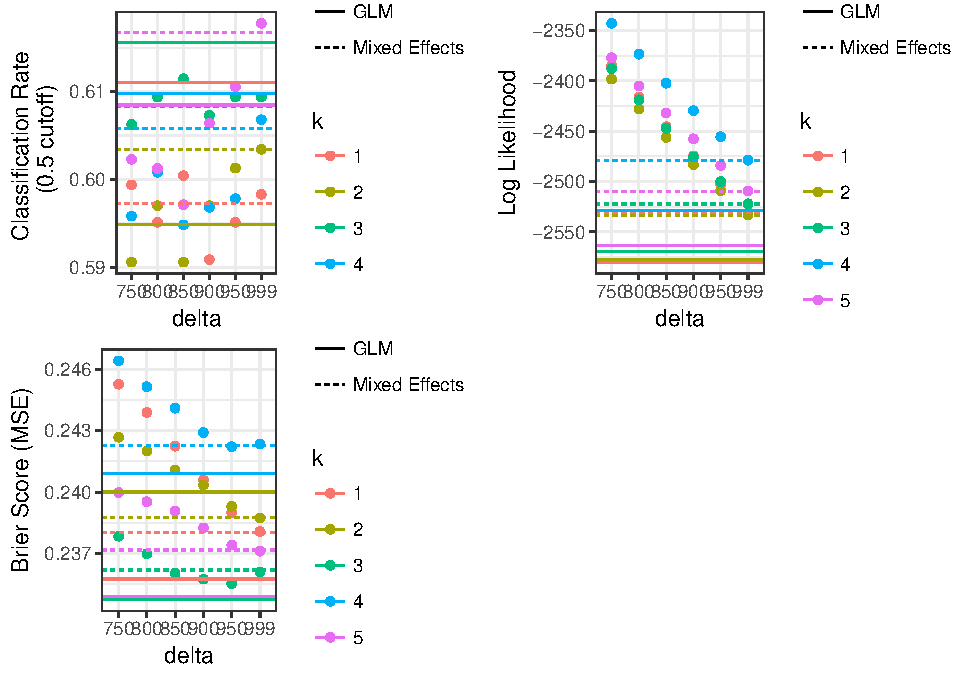
\includegraphics{thesis_files/figure-latex/home-1.pdf}

\section{2015 Season Only}\label{season-only}

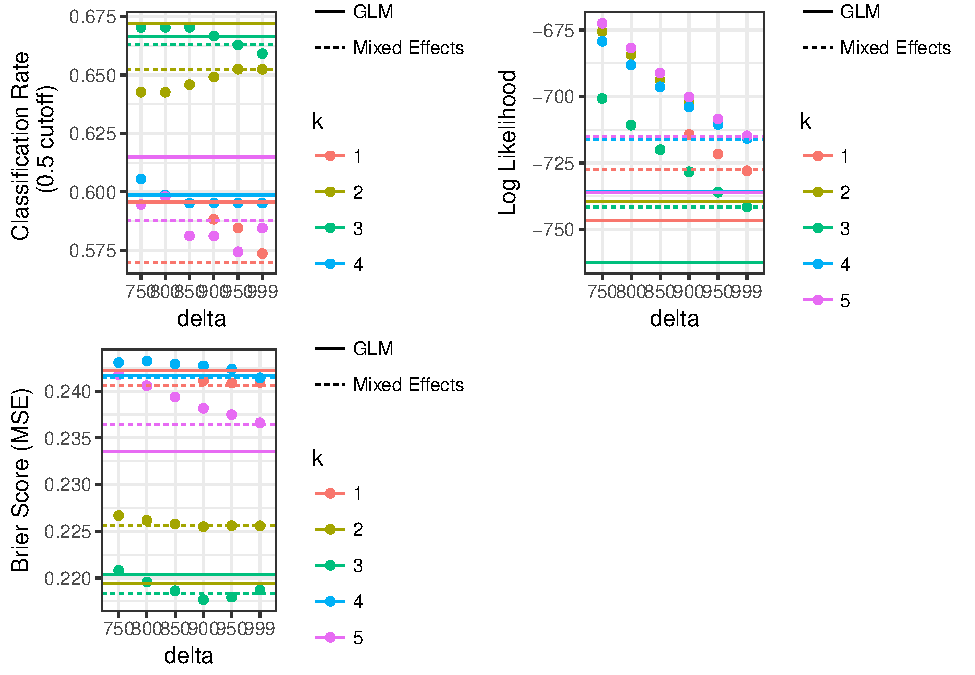
\includegraphics{thesis_files/figure-latex/2015-1.pdf}

\backmatter

\chapter*{References}\label{references}
\addcontentsline{toc}{chapter}{References}

\markboth{References}{References}

\noindent

\setlength{\parindent}{-0.20in} \setlength{\leftskip}{0.20in}
\setlength{\parskip}{8pt}

\hypertarget{refs}{}
\hypertarget{ref-albert93}{}
Albert, J. (1993). Statistical analysis of hitting streaks in baseball:
Comment. \emph{Journal of the American Statistical Association},
\emph{88}(424), 1184--1188.

\hypertarget{ref-albert13}{}
Albert, J. (2013). Looking at spacings to assess streakiness.
\emph{Journal of Quantitative Analysis in Sports}, \emph{9}(2), 1--13.

\hypertarget{ref-albert99}{}
Albert, J., \& Williamson, P. (1999). Using model/data simulations to
detect streakiness. \emph{The American Statistician}, \emph{55}, 41--50.

\hypertarget{ref-ameen84}{}
Ameen, J. R., \& Harrison, P. J. (1984). Discount weighted estimation.
\emph{Journal of Forecasting}, \emph{3}, 285--296.

\hypertarget{ref-bareli06}{}
Bar-Eli, M., Avugos, S., \& Raab, M. (2006). Twenty years of ``hot
hand'' research: Review and critique. \emph{Psychology of Sport and
Exercise}, \emph{7}, 525--553.

\hypertarget{ref-gilovich85}{}
Gilovich, T., Vallone, R., \& Tversky, A. (1985). The hot hand in
basketball: On the misperception of random sequences. \emph{Cognitive
Psychology}, \emph{17}, 295--314.

\hypertarget{ref-west10}{}
Prado, R., \& West, M. (2010). \emph{Time series: Modelling, computation
\& inference}. Chapman \& Hall/CRC Press.

\hypertarget{ref-wetzels16}{}
Ryan Wetzels, e. a. (2016). A bayesian test for the hot hand phenomenon.
\emph{Journal of Mathematical Psychology}, \emph{72}, 200--209.


% Index?

\end{document}
